\chapter{直线}\label{chp:line}
\section{有向线段、定比分点}
\subsection{有向线段、两点的距离}
在初中,我们学过数轴,它是规定了原点、正方向和长度单位的直线。
任意一条直线,都可以规定两个相反的方向。
如果把其中一个作为正方向,那么相反的方向就是负方向。
规定了正方向的直线叫做\Concept{有向直线}。
在图中,有向直线 $l$ 的正方向用箭头表示(\cref{fig:1-1})。
例如,初中学过的直角坐标系中的 $x$ 轴、 $y$ 轴都是有向直线。
\begin{figure}
  \begin{minipage}[b]{0.48\linewidth}\centering
    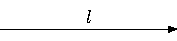
\includegraphics{1-1.pdf}
    \caption{}\label{fig:1-1}
  \end{minipage}
  \begin{minipage}[b]{0.48\linewidth}\centering
    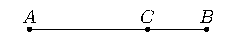
\includegraphics{1-2.pdf}
    \caption{}\label{fig:1-2}
  \end{minipage}
\end{figure}

一条线段也可以规定两个相反的方向。
如\cref{fig:1-2} 中的线段 $AB$,如果以 $A$ 为起点、$B$ 为终点,那么,它的方向是从 $A$ 到 $B$;相反,如果以 $B$ 为起点、$A$ 为终点,它的方向就是从 $B$ 到 $B$。
规定了方向,即规定了起点和终点的线段叫做\Concept{有向线段}。
表示有向线段时,要将表示起点的字母写在前面,表示终点的字母写在后面。
如以 $A$ 为起点、$B$ 为终点的有向线段记作 $\overline{AB}$。
\cref{fig:1-2} 中,点 $C$ 是线段 $AB$ 上的一点,$\overline{AB}$ 和 $\overline{AC}$ 是方向相同的有向线段,$\overline{AB}$ 和 $\overline{BC}$ 是方向相反的有向线段。

选定一条线段作为长度单位,我们可以量得一条线段的长度,线段 \({AB}\) 的长度,就是有向线段 $\overline{AB}$ 的长度,记作 $|AB|$。
如\cref{fig:1-3},设线段 $e$ 是长度单位,那么 $|AB|=3$。
因为有向线段的长度与它的方向无关,所以 $|AB|=|BA|$。
\begin{figure}
  \begin{minipage}[b]{0.48\linewidth}\centering
    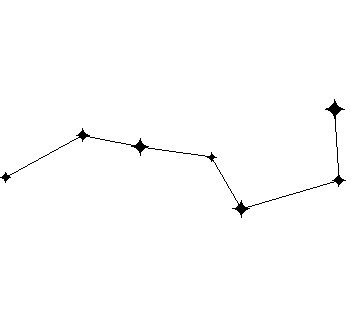
\includegraphics{1-3.pdf}
    \caption{}\label{fig:1-3}
  \end{minipage}
  \begin{minipage}[b]{0.48\linewidth}\centering
    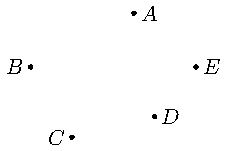
\includegraphics{1-4.pdf}
    \caption{}\label{fig:1-4}
  \end{minipage}
\end{figure}

如果有向线段在有向直线 $l$ 上或与 $l$ 平行,那么,它的方向与 $l$ 的正方向可能相同或相反。
例如\cref{fig:1-4} 中的 $\overline{AB}$ 与 $l$ 的方向相同,而 $\overline{BA}$ 与 $l$ 的方向相反.

根据 $\overline{AB}$ 与有向直线 $l$ 的方向相同或相反,分别把它的长度加上正号或负号,这样所得的数,叫做有向线段的\Concept{数量}(或\Concept{数值})。
有向线段 $\overline{AB}$ 的数量用 $AB$ 表示\footnote{在引入有向直线以后,线段 $AB$ 的长度一律用 $|AB|$ 表示。}、显然
\[AB = - BA.\]

数轴 $Ox$ 是有向直线,数轴上点 $P$ 的坐标 $x_0$ 实际上是以有向线段的数量来定义的。
点 $P$ 的坐标 $x_0$ 是以原点 $O$ 为起点、$P$ 为终点的有向线段 $\overline{OP}$ 的数量,$OP=x_0$。
例如,点 $A$、$B$ 的坐标分别是有向线段 $\overline{OA}$、$\overline{OB}$ 的数量,$OA=3$、$OB=-2$(\cref{fig:1-5})。
\begin{figure}
    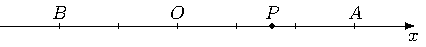
\includegraphics{1-5.pdf}
    \caption{}\label{fig:1-5}
\end{figure}

现在我们来研究,对于数轴上任意一条有向线段,怎样用它的起点坐标和终点坐标表示它的数量。

设 $\overline{AB}$ 是 $x$ 轴上的任意一条有向线段,$O$ 是原点。
先讨论两点 $A$、$B$ 与 $O$ 都不重合的情形。
如\cref{fig:1-6},它们的位置关系只可能有六种不同情形。
点 $O$、$B$ 的坐标分别用 $x_1$ 和 $x_2$ 表示,那么 $OA=x_1$,$OB=x_2$。

\begin{figure}
  \begin{minipage}{0.1\linewidth}
    \subcaption{}\label{fig:1-6a}
  \end{minipage}%
  \begin{minipage}{0.5\linewidth}
    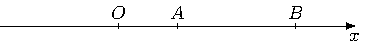
\includegraphics{1-6a.pdf}
  \end{minipage}\par
  \begin{minipage}{0.1\linewidth}
    \subcaption{}\label{fig:1-6b}
  \end{minipage}%
  \begin{minipage}{0.5\linewidth}
    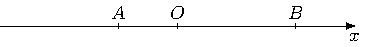
\includegraphics{1-6b.pdf}
  \end{minipage}\par
  \begin{minipage}{0.1\linewidth}
    \subcaption{}\label{fig:1-6c}
  \end{minipage}%
  \begin{minipage}{0.5\linewidth}
    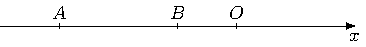
\includegraphics{1-6c.pdf}
  \end{minipage}\par
  \begin{minipage}{0.1\linewidth}
    \subcaption{}\label{fig:1-6d}
  \end{minipage}%
  \begin{minipage}{0.5\linewidth}
    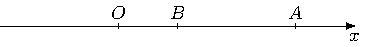
\includegraphics{1-6d.pdf}
  \end{minipage}\par
  \begin{minipage}{0.1\linewidth}
    \subcaption{}\label{fig:1-6e}
  \end{minipage}%
  \begin{minipage}{0.5\linewidth}
    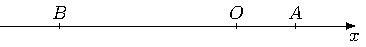
\includegraphics{1-6e.pdf}
  \end{minipage}\par
  \begin{minipage}{0.1\linewidth}
    \subcaption{}\label{fig:1-6f}
  \end{minipage}%
  \begin{minipage}{0.5\linewidth}
    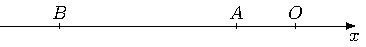
\includegraphics{1-6f.pdf}
  \end{minipage}\par
  \caption{}\label{fig:1-6}
\end{figure}

在\cref{fig:1-6a} 中,$AB=|AB|$,$OA=|OA|$,$OB=|OB|$,而 $|AB|=|OB|-|OA|$,

$\therefore AB=OB-OA$,即 $AB=x_2-x_1$。

在\cref{fig:1-6b} 中,$AB=|AB|$,$OA=-|OA|$,$OB=|OB|$,而 $|AB|=|OB|+|OA|$,

$\therefore AB=OB-OA$,即 $AB=x_2-x_1$。

同样可以证明,对于其他四种情况,这个等式也成立。
容易验证,当点 $A$ 或点 $B$ 与原点 $O$ 重合时这个等式同样成立。
因此,对于数轴上任意有向线段 $\overline{AB}$,它的数量 $AB$ 和起点坐标 $x_1$、终点坐标 $x_2$ 有如下关系:
\[ \tcbhighmath{AB = x_2 - x_1}. \]

根据这个公式可以得到,数轴上两点 $A$、$B$ 的距离公式
\[ |AB| = |x_2 - x_1| \]

\medskip\noindent
\begin{minipage}{0.67\linewidth}\parindent2em
下面,我们来求平面上任意两点的距离。

在直角坐标系中,已知两点 $P_1\,(x_1,y_1)$、$P_2\,(x_2,y_2)$(\cref{fig:1-7})。
从 $P_1$、$P_2$ 分别向 $x$ 轴和 $y$ 轴作垂线 $P_1M_1$、$P_1N_1$ 和 $P_2M_2$、$P_2N_2$,垂足分别为 $M_1\,(x_1,0)$、$N_1\,(0,y_1)$、$M_2\,(x_2,0)$、$N_2\,(0,y_2)$,其中直线 $P_1N_1$ 和 $P_2M_2$ 相交于点 $Q$。

在 Rt$\triangle P_1QP_2$ 中,
\begin{align*}
  |P_1P_2|^2 & = |P_1Q|^2+|QP_2|^2,\\
  \because \quad |P_1Q| &= |M_1M_2|=|x_2-x_1|,\\
  |QP_2| & = |N_1N_2|=|y_2-y_1|,\\
  \therefore \quad |P_1P_2|^2 &= |x_2-x_1|^2+|y_2-y_1|^2.
\end{align*}
\end{minipage}\hfill
\begin{minipage}{0.28\linewidth}\centering
\begin{figurehere}
  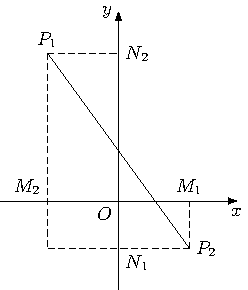
\includegraphics{1-7.pdf}
  \caption{}\label{fig:1-7}
\end{figurehere}
\end{minipage}

由此得到两点 $P_1\,(x_1,y_1)$、$P_2\,(x_2,y_2)$ 的\Concept{距离公式}:
\[ \tcbhighmath{|P_1P_2| = \sqrt{|x_2-x_1|^2+|y_2-y_1|^2}}. \]

\begin{example}
已知数轴上三点 $A$、$B$、$C$ 的坐标分别是 $4$、$-2$、$-6$。
求 $\overline{AB}$、$\overline{BC}$、$\overline{CA}$ 的数量和长度(\cref{fig:1-8})。
\end{example}
\begin{figure}
  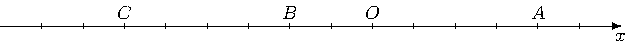
\includegraphics{1-8.pdf}
  \caption{}\label{fig:1-8}
\end{figure}
\begin{solution}
  \begin{align*}
    AB & = (-2)-4=-6,   & |AB| &=|-6|=6;\\
    BC & = -6-(-2)=-4,  & |BC| &=|-4|=4;\\
    CA & = 4-(-6)=-10,  & |CA| &=|10|=10.
  \end{align*}
\end{solution}

\begin{example}
  $\triangle ABC$ 中,$AO$ 是 $BC$ 边上的中线(\cref{fig:1-9})。求证:
  \[ |AB|^2 + |AC|^2 =2(|AO|^2+|OC|^2)\]
\end{example}
% \begin{figure}
%   \caption{}\label{fig:1-9}
% \end{figure}

\medskip\noindent
\begin{minipage}{0.67\linewidth}\parindent2em
\begin{proof}
  取线段 $BC$ 所在的直线为 $x$ 轴,点 $O$ 为原点建立直角坐标系。
  设点 $A$ 的坐标为 $(b,c)$,点 $C$ 的坐标为 $(a,0)$,则点 $B$ 的坐标为 $(-a,0)$。可得
  \begin{gather*}
  \begin{aligned}
    |AB|^2 &=(a+b)^2+c^2, & |AC|^2&=(a-b)^2+c^2,\\
    |AO|^2 &=b^2+c^2, & |OC|^2&=a^2.\\
  \end{aligned}\\
  \begin{aligned}
    \therefore\quad |AB|^2 +|AC|^2 &=2(a^2+b^2+c^2),\\
    |AO|^2 +|OC|^2 &=a^2+b^2+c^2.\\
    \therefore\quad |AB|^2 +|AC|^2 &=2(|AO|^2 +|OC|^2).
  \end{aligned}
\end{gather*}
\end{proof}
\end{minipage}\hfill
\begin{minipage}{0.28\linewidth}\centering
  \begin{figurehere}
    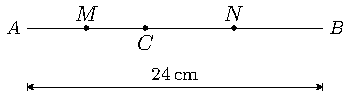
\includegraphics{1-9.pdf}
    \caption{}\label{fig:1-9}
  \end{figurehere}
\end{minipage}

\begin{Practice}
  \begin{question}
    \item 数轴上点 $A$ 的坐标为 2,点 $B$ 的坐标为 $-3$。验证公式 $AB=x_2-x_1$。
    \item 已知数轴 $x$ 上的点 $A$、$B$、$C$ 的坐标分别为 1、2、3。
    \begin{tasks}
      \task 求 $\overline{AB}$、$\overline{CB}$ 的数量;
      \task 如果在 $x$ 轴上还有两个点 $D$、$E$,且 $AD=2.5$,$CE=-3$。求点 $D$、$E$ 的坐标。
    \end{tasks}
    \item 求有下列坐标的两点距离:
    \begin{tasks}(2)
      \task  $(6,0)$、$(-2,0)$;
      \task  $(0,-4)$、$(0,-1)$;
      \task  $(6,0)$、$(0,-2)$;
      \task  $(2,1)$、$(5,-1)$;
      \task  $\left(\dfrac{\sqrt{3}}{2},-\dfrac{\sqrt{2}}{2}\right)$、$\left(-\dfrac{\sqrt{2}}{2},-\dfrac{\sqrt{3}}{2}\right)$;
      \task  $(ab^2,2abc)$、$(ac^2,0)$。
    \end{tasks}
    \item 已知点 $A\,(a,-5)$ 和 $A\,(0,10)$ 的距离是 17,求 $a$ 的值。
  \end{question}
\end{Practice}

\subsection{线段的定比分点}
有向直线 $l$ 上的一点 $P$,把 $l$ 上的有向线段 $\overline{P_1P_2}$ 分成两条有向线段 $\overline{P_1P}$ 和 $\overline{PP_2}$。$\overline{P_1P}$ 和 $\overline{PP_2}$ 数量的比叫做\Concept{点 $P$ 分 $\overline{P_1P_2}$ 所成的比},通常用字母 $\lambda$ 来表示这个比值,
\[ \lambda = \frac{P_1P}{PP_2} \]

点 $P$ 叫做 $\overline{P_1P_2}$ 的\Concept{定比分点}。

如果点 $P$ 在线段 $\overline{P_1P_2}$ 上(\cref{fig:1-10a}),点 \(P\) 叫做 \(\overline{{P}_{1}{P}_{2}}\) 的\Concept{内分点}。
这时,无论 $l$ 的方向如何,$\overline{P_1P}$ 和 $\overline{PP_2}$ 的方向都相同,它们的数量的符号也相同,所以 $\lambda$ 为正值。
如果点 $P$ 在线段 $\overline{P_2P_1}$ 或 $\overline{P_1P_2}$ 的延长线上(\cref{fig:1-10b,fig:1-10c}),点 $P$ 叫做 $\overline{P_1P_2}$ 的\Concept{外分点}。
\begin{figure}
  \begin{minipage}{0.1\linewidth}
    \subcaption{}\label{fig:1-10a}
  \end{minipage}%
  \begin{minipage}{0.5\linewidth}
    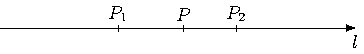
\includegraphics{1-10a.pdf}
  \end{minipage}\par
  \begin{minipage}{0.1\linewidth}
    \subcaption{}\label{fig:1-10b}
  \end{minipage}%
  \begin{minipage}{0.5\linewidth}
    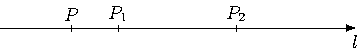
\includegraphics{1-10b.pdf}
  \end{minipage}\par
  \begin{minipage}{0.1\linewidth}
    \subcaption{}\label{fig:1-10c}
  \end{minipage}%
  \begin{minipage}{0.5\linewidth}
    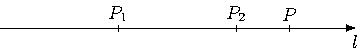
\includegraphics{1-10c.pdf}
  \end{minipage}
  \caption{}\label{fig:1-10}
\end{figure}
这时无论 $l$ 的方向如何,$\overline{P_1P}$ 和 $\overline{PP_2}$ 的方向都相反,它们的数量的符号也相反,所以 $\lambda$ 为负值。

由于点 $P$ 分 $\overline{P_1P_2}$ 所成的比与它们所在的直线 $l$ 的方向无关,为了简便起见,在以后谈到点 $P$ 分 $\overline{P_1P_2}$ 所成的比时,一般不提它所在的有向直线的方向。

\medskip\noindent
\begin{minipage}{0.58\linewidth}\parindent2em
设 $\overline{P_1P_2}$ 的两个端点分别为 $P_1\,(x_1,y_1)$ 和 $P_2\,(x_2,y_2)$,点 $P$ 分 $\overline{P_1P_2}$ 所成的比为 $\lambda(\lambda\neq-1)$(\cref{fig:1-11}),求分点 $P$ 的坐标 $(x,y)$。

过点 $P_1$、$P_2$、$P$ 分别作 $x$ 轴的垂线 $P_1M_1$、$P_2M_2$、$PM$,则垂足分别为 $M_1\,(x_1,0)$、$M_2\,(x_2,0)$、$M\,(x,0)$。根据平行线分线段成比例定理,得
\[ \frac{|P_1P|}{|PP_2|}=\frac{|M_1M|}{|MM_2|}. \]
\end{minipage}\hfill
\begin{minipage}{0.37\linewidth}\centering
\begin{figurehere}
  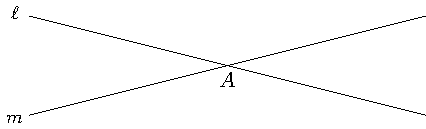
\includegraphics{1-11.pdf}
  \caption{}\label{fig:1-11}
\end{figurehere}
\end{minipage}

\medskip
{\linespread{1.6}\selectfont 如果点 $P$ 在线段 $P_1P_2$ 上,那么点 $M$ 也在线段 $M_1M_2$ 上;如果点 $P$ 在线段 $P_1P_2$ 或 $P_2P_1$ 的延长线上,那么点 $M$ 也在线段 $M_1M_2$ 或 $M_2M_1$ 的延长线上。
因此 $\dfrac{|P_1P|}{|PP_2|}$ 与 $\dfrac{|M_1M|}{|MM_2|}$ 的符号相同,所以\par}
\begin{align*}
  \frac{P_1P}{PP_2}&=\frac{M_1M}{MM_2}.\\
  \because \quad M_1M&=x-x_1, \\
  MM_2&=x_2-x, \\
  \therefore \quad \lambda&=\frac{x-x_1}{x_2-x} 
\end{align*}
即 $(1+\lambda)x=x_1+\lambda x_2$,当 $\lambda\neq -1$ 时,得
\[ x= \frac{x_1+\lambda x_2}{1+\lambda}.\]

同理可以求得
\[ \lambda=\frac{y-y_1}{y_2-y}, \quad y=\frac{y_1+\lambda y_2}{1+\lambda}.\]

因此,当已知两个端点为 $P_1\,(x_1,y_1)$、$P_2\,(x_2,y_2)$,点 $P\,(x,y)$ 分 $\overline{P_1P_2}$ 所成的比为 $\lambda$ 时,点 $P$ 的坐标是
\[ \tcbhighmath{x= \frac{x_1+\lambda x_2}{1+\lambda}, \quad y=\frac{y_1+\lambda y_2}{1+\lambda}\,(\lambda\neq-1)}.\]

当点 $P$ 是线段 $\overline{P_1P_2}$ 的中点时,有 $P_1P=PP_2$,即 $\lambda = 1$。
因此线段 $\overline{P_1P_2}$ 中点 $P$ 的坐标是
\[ \tcbhighmath{x=\frac{x_1+x_2}{2},\quad y=\frac{y_1+y_2}{2}}.\]
\begin{example}
点 $P_1$ 和 $P_1$ 的坐标分别是 $(-1,-6)$ 和 $(3,0)$,点 $P$ 的横坐标为 $-\dfrac{7}{3}$。求点 $P$ 分 $\overline{P_1P_2}$ 所成的比 $\lambda$ 和点 $P$ 的纵坐标 $y$。
\end{example}
\noindent
\begin{minipage}{0.65\linewidth}\parindent2em
\begin{solution}
  由 $\lambda$ 的定义,可得
  \begin{gather*} 
    \lambda=\frac{x-x_1}{x_2-x}=\frac{-\dfrac{7}{3}-(-1)}{3-\left(-\dfrac{7}{3}\right)}=-\frac{1}{4}.\\
    y=\frac{y_1+\lambda y_2}{1+\lambda}=\frac{-6+ \left( -\dfrac{1}{4}\right)\cdot 0}{1+\left( -\dfrac{1}{4}\right)}=-8.
  \end{gather*}

  点 $P$ 分 $\overline{P_1P_2}$ 所成的比是 $-\dfrac{1}{4}$ ,点 $P$ 的纵坐标是 $-8$(\cref{fig:1-12})。
\end{solution}
\end{minipage}\hfill
\begin{minipage}{0.3\linewidth}\centering
\begin{figurehere}
  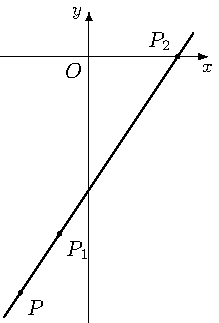
\includegraphics{1-12.pdf}
  \caption{}\label{fig:1-12}
\end{figurehere}
\end{minipage}

\medskip
\begin{example}
  已知三角形顶点是 $A\,(x_1,y_1)$、$B\,(x_2,y_2)$、$C\,(x_3,y_3)$。求 $\triangle ABC$ 的重心 $G$ 的坐标 $(x,y)$ (\cref{fig:1-13})。
\end{example}
\noindent
\begin{minipage}{0.65\linewidth}\parindent2em
\begin{solution}
  设 $BC$ 边的中点为 $D$,则点 $D$ 的坐标是
  \[ \left(\frac{x_2+x_3}{2},\frac{y_2+y_3}{2}\right).\]
  又因为 $AD$ 是中线,且 $\dfrac{AG}{GD} = 2$,所以点 $G$ 的坐标是
  \[
    x=\frac{x_1+2\times\dfrac{x_2+x_3}{2}}{1+2},\quad
    y=\frac{y_1+2\times\dfrac{y_2+y_3}{2}}{1+2}, 
  \]
\end{solution}
\end{minipage}\hfill
\begin{minipage}{0.3\linewidth}\centering
\begin{figurehere}
  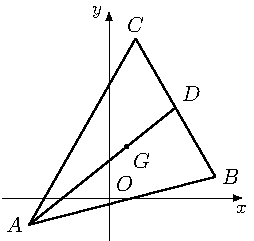
\includegraphics{1-13.pdf}
  \caption{}\label{fig:1-13}
\end{figurehere}
\end{minipage}

\medskip\noindent
整理后得重心 \(G\) 的坐标
  \[ x=\frac{x_1+x_2+x_3}{3},\quad y=\frac{y_1+y_2+y_3}{3}.\]

\begin{Practice}
  \begin{question}
    \item 已知两点 $P_1\,(3,-2)$、$P_2\,(-9,4)$。求点 $P\,(x,0)$ 分 $\overline{P_1P_2}$ 所成的比 $\lambda$ 及 $x$ 的值。
    \item 点 $M$ 分有向线段 $\overline{M_1M_2}$ 的比为 $\lambda$,求点 $M$ 的坐标 $(x,y)$:
    \begin{tasks}
      \task 已知:$M_1\,(1,5)$、$M_2\,(2,3)$,$\lambda = \dfrac{1}{3}$;
      \task 已知:$M_1\,(1,5)$、$M_2\,(2,3)$,$\lambda = -2$;
      \task 已知:$M_1\,(1,5)$、$M_2\,(2,-3)$,$\lambda = -2$;
    \end{tasks}
    \item 已知 $\triangle ABC$ 的顶点 $A\,(2,3)$、$B\,(8,-4)$ 和重心 $G\,(2,-1)$。求点 $C$ 的坐标 $(x,y)$。
  \end{question}
\end{Practice}

\begin{Exercise}
  \begin{question}
    \item\label{exer:1-1} 如图,数轴上每一格等于一个长度单位,说出有向线段 $\overline{AB}$、$\overline{BC}$、$\overline{CD}$ 和 $\overline{EA}$ 的长度和数量。
    \begin{figurehere}
      \begin{minipage}{\linewidth}\centering
        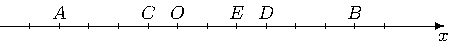
\includegraphics{ex1-1.pdf}
        \caption*{(第 \ref{exer:1-1} 题)}
      \end{minipage}
    \end{figurehere}
    \item 已知数轴上 $A$、$B$ 两点的坐标 $x_1$、$x_2$ 分别是:
    \begin{tasks}(2)
      \task $x_1=8$,$x_2=6$;
      \task $x_1=5$,$x_2=-3$;
      \task $x_1=-4$,$x_2=0$;
      \task $x_1=-9$,$x_2=-1$;
      \task $x_1=2a-b$,$x_2=a-2b$;
      \task $x_1=2+\sqrt{3}$,$x_2=3+\sqrt{2}$。
    \end{tasks}
    求 $\overline{AB}$ 和 $\overline{BA}$ 的数量。
    \item $A$、$B$ 是数轴上两点,点 $B$ 的坐标是 $x_2$。根据下列条件,求点 $A$ 的坐标 $x_1$:
    \begin{tasks}(2)
      \task $x_2=3$,$AB=5$;
      \task $x_2=-5$,$BA=-3$;
      \task $x_2=0$,$|AB|=2$;
      \task $x_2=-5$,$|AB|=2$。
    \end{tasks}
    \item 已知某零件一个面上有 3 个孔,孔中心的坐标分别为:$A\,(-10,30)$、$B\,(-2,3)$、$C\,(0,-1)$。求每两孔中心的距离。
    \item 已知点 $P\,(x,2)$、$Q\,(-2,-3)$、$M\,(1,1)$,且 $|PQ|=|PM|$。求 $x$。
    \item 解答:
    \begin{enumerate}[itemindent=2em]
      \item 求在 $x$ 轴上与点 $A\,(5,12)$ 的距离为 $13$ 的点的坐标;
      \item 已知点 $P$ 的横坐标是 7,点 $P$ 到点 $N\,(-1,5)$ 的距离等于 10,求点 $P$ 的纵坐标。
    \end{enumerate}
    \item 设线段 $P_1P_2$ 长 \qty{5}{cm},写出点 $P$ 分 $\overline{P_1P_2}$ 所成的比 $\lambda$:
    \begin{tasks}
      \task 点 $P$ 在 $P_1P_2$ 上,$|P_1P|=\qty{1}{cm}$;
      \task 点 $P$ 在 $P_1P_2$ 的延长线上,$|P_2P|=\qty{10}{cm}$;
      \task 点 $P$ 在 $P_1P_1$ 的延长线上,$|PP_1|=\qty{1}{cm}$。
    \end{tasks}
    \item 求连结下列两点的线段的长度和中点坐标:
    \begin{tasks}(2)
      \task $A\,(7,4)$、$B\,(3,2)$;
      \task $A\,(6,-4)$、$B\,(-2,-2)$;
      \task $M\,(3,1)$、$N\,(2,1)$;
    \end{tasks}
    \item 一条线段的两个端点 $P_1$、$P_1$ 的坐标及点 $P$ 分 $\overline{P_1P_2}$ 所成的比如下,求分点 $P$ 的坐标:
    \begin{tasks}(2)
      \task $(2,1)$、$(3,-9)$,$\lambda=4$;
      \task $(5,-2)$、$(5,3)$,$\lambda=-\dfrac{2}{3}$;
      \task $(-4,1)$、$(5,4)$,$\lambda=\dfrac{5}{2}$;
      \task $(8,5)$、$(-13,-2)$,$\lambda=-\dfrac{4}{3}$。
    \end{tasks}
    \item 解答:
    \begin{enumerate}[itemindent=2em]
      \item 一条线段的两个端点坐标如下,求这条线段的两个三等分点的坐标:
      \begin{tasks}(2)
        \task $(-1,2)$、$(10,-1)$;
        \task $(7,8)$、$(1,-6)$。
      \end{tasks}
      \item 已知点 $A\,(1,-1)$、$B\,(-4,5)$。将线段 $AB$ 延长至 $C$,使 $|AC|=3|AB|$。求点 $C$ 的坐标。
    \end{enumerate}
    \item 三角形的三个顶点是 $A\,(2,1)$、$B\,(-2,3)$、$C\,(0,-1)$。求三条中线的长度。
    \item 已知点 $P_1$ 和 $P_2$ 的坐标分别是 $(4,-3)$ 和 $(-2,6)$,求适合下列条件的点 $P$ 的坐标:
    \begin{tasks}
      \task $\dfrac{|P_1P|}{|PP_2|}=2$,点 $P$ 在线段 $P_1P_2$ 上。
      \task $\dfrac{|P_1P|}{|PP_2|}=4$,点 $P$ 在线段 $P_1P_2$ 的延长线上。
      \task $\dfrac{|P_1P|}{|PP_2|}=\dfrac{4}{5}$,点 $P$ 在线段 $P_2P_1$ 的延长线上。
    \end{tasks}
    \item 解答:
    \begin{tasks}
      \task 已知三点 $A\,(x,5)$、$B\,(-2,y)$、$C\,(1,1)$,且点 $C$ 平分线段 $AB$。求 $x$、$y$。
      \task 已知三点 $A\,(3,-1)$、$B\,(2,1)$,求点 $A$ 关于点 $B$ 的对称点的坐标。
    \end{tasks}
    \item 已知三点 $A\,(1,-1)$、$B\,(3,3)$、$C\,(4,5)$。求证:三点在一条直线上。
    \item 证明:
    \begin{tasks}
      \task 直角三角形斜边的中点到三个顶点的距离相等;
      \task 三角形中位线等于底边的一半。
    \end{tasks}
  \end{question}
\end{Exercise}

\section{直线的方程}
\subsection{一次函数的图像与直线的方程}
\noindent
\begin{minipage}{0.65\linewidth}\parindent2em
初中研究一次函数时,在直角坐标系中,画出的一次函数图象是一条直线。
例如函数 $y=2x+1$ 的图象是直线 $l$(\cref{fig:1-14})。
这时,满足函数式 $y=2x+1$ 的每一对 $x$、$y$ 的值都是直线 $l$ 上的点的坐标,如数对 $(0,1)$ 满足函数式,在直线 $l$ 上就有一点 $A$,它的坐标是 $(0,1)$;而直线  $l$ 上每一点的坐标都满足函数式,如直线 $l$ 上点 $P$ 的坐标是 $(1,3)$,数对 $(1,3)$ 就满足函数式。
\end{minipage}\hfill
\begin{minipage}{0.3\linewidth}\centering
\begin{figurehere}
  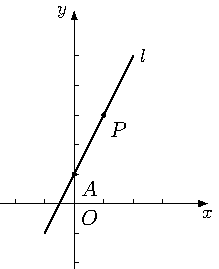
\includegraphics{1-14.pdf}
  \caption{}\label{fig:1-14}
\end{figurehere}
\end{minipage}

\medskip
一般地,一次函数 $y=kx+b$ 的图象是一条直线,它是以满足 $y=kx+b$ 的每一对 $x$、$y$ 的值为坐标的点构成的。
由于函数 $y=kx+b$ 也可以看作二元一次方程,因此,我们也可以说,这个方程的解和直线上的点也存在这样的一一对应关系。

以一个方程的解为坐标的点都是某条直线上的点;反之,这条直线上点的坐标都是这个方程的解,这时,这个方程就叫做这条直线的方程,这条直线叫做这个方程的直线。

在解析几何里研究直线时,就是利用直线与方程的这种关系,建立直线的方程,并通过方程来研究直线的有关问题。

\begin{Practice}
  \begin{question}
    \item 在坐标平面上,画出下列方程的直线:
    \begin{tasks}(2)
      \task $y=x$;
      \task $2x+y=6$;
      \task $2x+3y+6=0$;
      \task $2x-3y+6=0$。
    \end{tasks}
    \item 解答:
    \begin{tasks}
      \task 用量角器测量上题中各直线向上的方向与 $x$ 轴的正方向所成的角的度数;
      \task 量出各直线与 $x$ 轴、$y$ 轴交点的坐标,并代入方程,看它们是不是方程的解。
    \end{tasks}
  \end{question}
\end{Practice}

\subsection{直线的倾斜角和斜率}
为了建立直角坐标系中的直线方程,需要研究直线的倾斜角和斜率。

一条直线 $l$ 向上的方向与 $x$ 轴的正方向所成的最小正角叫做这条直线的倾斜角,如\cref{fig:1-15} 中的 $\alpha$。特别地,当直线 $l$ 和 $x$ 轴平行时,我们规定它的倾斜角为 \ang{0}。因此,倾斜角的取值范围是 $\ang{0}\leqslant\alpha<\ang{180}$。
\begin{figure}
  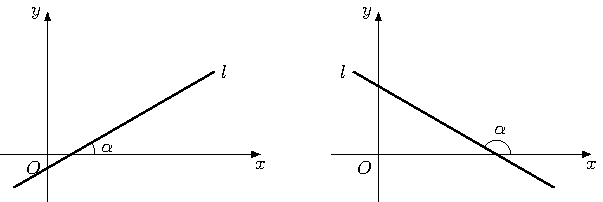
\includegraphics{1-15.pdf}
  \caption{}\label{fig:1-15}
\end{figure}

倾斜角不是 \ang{90} 的直线,它的倾斜角的正切叫做这条直线的\Concept{斜率}。
直线的斜率常用 $k$ 表示,即
\[ \tcbhighmath{k = \tan\alpha}. \]

倾斜角是 \ang{90} 的直线没有斜率;倾斜角不是 \ang{90} 的直线,都有斜率,并且是确定的,我们常用斜率来表示倾斜角不等于 \ang{90} 的直线对于 $x$ 轴的倾斜程度。

在坐标平面上,如果已知两点 $P_1\,(x_1,x_1)$、$P_2\,(x_2,x_2)$,那么直线 $P_1P_2$ 就是确定的,当直线 $P_1P_2$ 的倾斜角不等于 \ang{90} 时,这条直线的斜率也是确定的。
下面我们来研究怎样用两点的坐标来表示直线 $P_1P_2$ 的斜率。

设直线 $P_1P_2$ 的倾斜角是 $\alpha$,斜率是 $k$,$\overline{P_1P_2}$ 的方向是向上的方向。
从 $P_1$、$P_2$ 分别向 $x$ 轴作垂线 $P_1M_1$、$P_2M_2$,再作 $P_1Q \perp P_2M_2$,垂足分别是 $M_1$、$M_2$、$Q$。那么 $\alpha = \angle QP_1P_2$(\cref{fig:1-16a}),或 $\alpha = \angle PP_1P_2$(\cref{fig:1-16b})。
\begin{figure}
  \begin{minipage}[b]{0.48\linewidth}\centering
    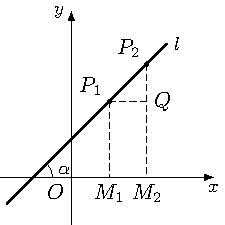
\includegraphics{1-16a.pdf}
    \subcaption{}\label{fig:1-16a}
  \end{minipage}
  \begin{minipage}[b]{0.48\linewidth}\centering
    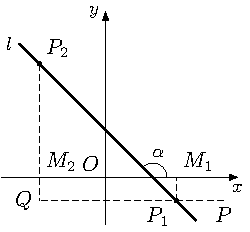
\includegraphics{1-16b.pdf}
    \subcaption{}\label{fig:1-16b}
  \end{minipage}
  \caption{}\label{fig:1-16}
\end{figure}

在\cref{fig:1-16a} 中,
\[ \tan\alpha =\tan\angle QP_1P_2 =\frac{QP_2}{P_1Q}=\frac{y_2-y_1}{x_2-x_1}.\]

在\cref{fig:1-16a} 中,
\[ \tan\alpha =\tan\angle PP_1P_2 =\frac{QP_2}{P_1Q}=\frac{y_2-y_1}{x_2-x_1}.\]

同样,对于 $\overline{P_2P_1}$ 方向向上的情形,
\[ \tan\alpha= \frac{y_1-y_2}{x_1-x_2}=\frac{y_2-y_1}{x_2-x_1}. \]

综上所述,我们得到经过点 $P_1\,(x_1,x_1)$、$P_2\,(x_2,x_2)$ 两点的直线的斜率公式:
\[ \tcbhighmath{k=\frac{y_2-y_1}{x_2-x_1}}. \]
\begin{example}
如\cref{fig:1-17},直线 $l_1$ 的倾斜角 $\alpha_1=\ang{30}$,直线 $l_2 \perp l_1$。求 $l_1$、$l_2$ 的斜率。
\end{example}
\noindent
\begin{minipage}{0.55\linewidth}\parindent2em
\begin{solution}
  $l_1$ 的斜率 $k_1=\tan\ang{30}=\dfrac{\sqrt{3}}{3}$,

  $\because\quad l_2$ 的倾斜角 
  \[\alpha_2=\ang{90}+\ang{30}=\ang{120},\]

  $\therefore\quad l_2$ 的斜率 
  \[k_2=\tan\ang{120}=-\tan\ang{60}=-\sqrt{3}.\]
\end{solution}
\end{minipage}\hfill
\begin{minipage}{0.4\linewidth}\centering
\begin{figurehere}
    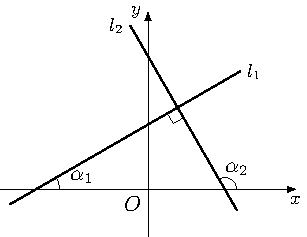
\includegraphics{1-17.pdf}
    \caption{}\label{fig:1-17}
\end{figurehere}
\end{minipage}
\begin{example}
求经过 $A\,(-2,0)$、$B\,(-5,3)$ 两点的直线的斜率和倾斜角。
\end{example}
\begin{solution}
\[ k=\frac{3-0}{-5-(-2)}=-1\]
就是:$\tan \alpha=-1$。

$\because\quad \ang{0}\leqslant\alpha<\ang{180}$,

$\therefore\quad \alpha=\ang{135}$。

因此,这条直线的斜率是 $-1$,倾斜角是 \ang{135}。
\end{solution}

\begin{Practice}
  \begin{question}
    \item 已知直线的倾斜角,讨论这条直线的斜率的值:
    \begin{tasks}(2)
      \task $\alpha=\ang{0}$;
      \task $\ang{0}<\alpha<\ang{90}$;
      \task $\alpha=\ang{90}$;
      \task $\ang{90}\alpha<\ang{180}$。
    \end{tasks}
    \item 求经过下列每两个点的直线的斜率和倾斜角:
    \begin{tasks}(2)
      \task $C\,(10,8)$、$D\,(4,-4)$;
      \task $P\,(0,0)$、$Q\,(-1,\sqrt{3})$;
      \task $M\,(-\sqrt{3},\sqrt{2})$、$N\,(-\sqrt{2},\sqrt{3})$。
    \end{tasks}
    \item 已知:$a$、$b$、$c$ 是两两不等的实数。求经过下列每两个点的直线的倾斜角:
    \begin{tasks}(2)
      \task $A\,(a,c)$、$B\,(b,c)$;
      \task $C\,(a,b)$、$D\,(a,c)$;
      \task $P\,(b,b+c)$、$Q\,(c,c+a)$。
    \end{tasks}
    \item 证明: 已知三点 $A$、$B$、$C$。如果直线 $AB$、$AC$ 的斜率相同。那么这三点在同一条直线上。
  \end{question}
\end{Practice}

\subsection{直线方程的几种形式}
一条直线在直角坐标平面内的位置,可以由不同的条件来确定。
下面,我们来研究怎样根据所给的条件,求出直线的方程。

\subsubsection{点斜式}
已知直线 $l$ 的斜率是 $k$,并且经过点 $P_1\,(x_1,y_1)$,求直线 $l$ 的方程(图\cref{fig:1-18})。

设点 $P\,(x,y)$ 是直线 $l$ 上不同于点 $P_1$ 的任意一点。
根据经过两点的直线的斜率公式,得
\[k = \frac{y - y_1}{x - x_1} \]
可化为
\[\tcbhighmath{y - y_1= k(x - x_1)}.\]

\begin{figure}
  \begin{minipage}[b]{0.48\linewidth}\centering
    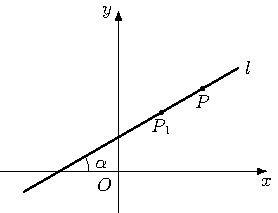
\includegraphics{1-18.pdf}
    \caption{}\label{fig:1-18}
  \end{minipage}
  \begin{minipage}[b]{0.48\linewidth}\centering
    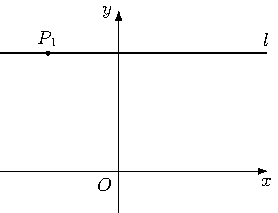
\includegraphics{1-19.pdf}
    \caption{}\label{fig:1-19}
  \end{minipage}
\end{figure}

可以验证,直线 $l$ 上的每个点的坐标都是这个方程的解;反过来,以这个方程的解为坐标的点都在直线 $l$ 上,所以这个方程就是过点 \({P}_{1}\) 、斜率为 $k$ 的直线 $l$ 的方程。

这个方程是由直线上一点和直线的斜率确定的,叫做直线方程的点斜式。

当直线 $l$ 的倾斜角为 \ang{0} 时(\cref{fig:1-19}),$\tan\ang{0}=0$,即 $k=0$。这时直线 $l$ 的方程就是
\[ y = y_1 \]

当直线 $l$ 的倾斜角为 \({90}^{ \circ }\) 时,直线没有斜率,这时直线 $l$ 与 \(y\) 轴平行或重合,它的方程不能用点斜式表示。但因 $l$ 上每一点的横坐标都等于 $x_1$(\cref{fig:1-20}),所以它的方程是
\[ x = x_1 \]

\begin{figure}
  \begin{minipage}[b]{0.48\linewidth}\centering
    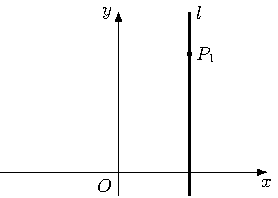
\includegraphics{1-20.pdf}
    \caption{}\label{fig:1-20}
  \end{minipage}
  \begin{minipage}[b]{0.48\linewidth}\centering
    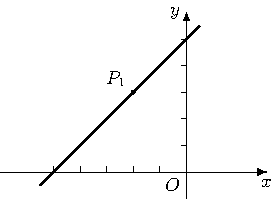
\includegraphics{1-21.pdf}
    \caption{}\label{fig:1-21}
  \end{minipage}
\end{figure}

\begin{example}
  一条直线经过点 $P_1\,(-2,3)$,倾斜角 $\alpha=\ang{45}$。求这条直线的方程,并画出图形。
\end{example}
\begin{solution}
  这条直线经过点 $P_1\,(-2,3)$,斜率是 
  \[k=\tan\ang{45}=1\]
  代入点斜式,得
  \[ y-3=x+2,\]
  即
  \[ x-y+5=0,\]
  这就是所求的直线方程,图形如\cref{fig:1-21}。
\end{solution}

如果已知直线 $l$ 的斜率是 $k$,与 $y$ 轴的交点是 $(0,b)$($b$ 是直线 $l$ 在 $y$ 轴上的截距),代入点斜式得直线 $l$ 的方程:
\[ y-b=k(x-0). \]
也就是
\[ \tcbhighmath{y=kx+b}. \]

这个方程是由直线 $l$ 的斜率和它在 $y$ 轴上的截距确定的,所以叫做直线方程的\Concept{斜截式}。

\begin{Practice}
  \begin{question}
    \item 写出下列直线的点斜式方程,并画出图形:
    \begin{tasks}
      \task 经过点 $A\,(2,5)$,斜率是 4 ;
      \task 经过点 $B\,(3,-1)$,斜率是 $\sqrt{2}$;
      \task 经过点 $C\,(-\sqrt{2},2)$,倾斜角是 \ang{30};
      \task 经过点 $D\,(0,3)$,倾斜角是 \ang{0};
      \task 经过点 $E\,(4,-2)$,倾斜角是 \ang{120}。
    \end{tasks}
    \item 已知下列直线的点斜式方程,求各直线经过的已知点、直线的斜率和倾斜角:
    \begin{tasks}(2)
      \task $y-2=x - 1$;
      \task $y-3=\sqrt{3}(x-4)$;
      \task $y+3=-(x-1)$;
      \task $y+2=-\dfrac{\sqrt{3}}{3}(x+1) $。
    \end{tasks}
    \item 写出下列直线的斜截式方程:
    \begin{tasks}
      \task 斜率是 $\dfrac{\sqrt{3}}{2}$,$y$ 轴上的截距是 $-2$;
      \task 倾斜角是 \ang{135},$y$ 轴上的截距是 3。
    \end{tasks}
  \end{question}
\end{Practice}

\subsubsection{两点式}
已知直线 $l$ 经过两点 $P_1\,(x_1,y_1)$、$P_2\,(x_2,y_2)$($x_1\neq x_2$),求直线 $l$ 的方程。

因为直线 $l$ 经过点 $P_1\,(x_1,y_1)$、$P_2\,(x_2,y_2)$,并且 $x_1\neq x_2$,所以它的斜率 
\[k = \frac{y_2-y_1}{x_2-x_1}.\] 
代入点斜式,得
\[ y-y_1 =\frac{y_2-y_1}{x_2-x_1}(x-x_1).\]
当 $y_2\neq y_1$ 时,方程可以写成:
\[ \tcbhighmath{\frac{y-y_1}{y_2-y_1} = \frac{x-x_1}{x_2-x_1}}.\]

这个方程是由直线上两点确定的,叫做直线方程的\Concept{两点式}。
\begin{example}
  已知直线 $l$ 在 $x$ 轴和 $y$ 轴上的截距分别是 $a$ 和 $b$ ($a\neq 0$,$b\neq 0$),求直线 $l$ 的方程。
\end{example}
\begin{solution}
  因为直线 $l$ 经过 $A\,(a,0)$ 和 $B\,(0,b)$ 两点,将这两点的坐标代入两点式,得
\[ \frac{y-0}{b-0} = \frac{x-a}{0-a} \]
就是
\[ \tcbhighmath{\frac{x}{a} + \frac{y}{b} = 1} \]
\end{solution}

这个方程是由直线在 $x$ 轴和 $y$ 轴上的截距确定的,叫做直线方程的\Concept{截距式}。
\begin{example}
  三角形的顶点是 $A\,(-5,0)$、$B\,(3,-3)$、$C\,(0,2)$(\cref{fig:1-22}),求这个三角形三边所在直线的方程。
\end{example}
\noindent
\begin{minipage}{0.55\linewidth}\parindent2em
\begin{solution}
  直线 $AB$ 过 $A\,(-5,0)$、$B\,(3,-3)$ 两点。由两点式得
  \[ \frac{y-0}{-3-0}=\frac{x-(-5)}{3-(-5)},\]
  即
  \[ 3x + 8y + 15 = 0 .\]

  这就是直线 $AB$ 的方程。
\end{solution}
\end{minipage}\hfill
\begin{minipage}{0.45\linewidth}\centering
  \begin{figurehere}
    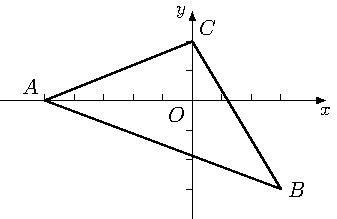
\includegraphics{1-22.pdf}
    \caption{}\label{fig:1-22}
  \end{figurehere}
\end{minipage}

\medskip
  直线 $BC$ 在 $y$ 轴上的截距是 2,斜率是
  \[ k=\frac{2-(-3)}{0-3}=-\frac{5}{3}. \]
  即
  \[ 5x + 3y - 6 = 0 .\]

  这就是直线 $BC$ 的方程。

  直线 $AC$ 在 $x$ 轴、$y$ 轴上的截距分别是 $-5$、2。由截距式得
  \[ \frac{x}{-5} + \frac{y}{2} = 1,\]
  即
  \[ 2x - 5y + 10 = 0 .\]

  这就是直线 $AC$ 的方程。

\begin{Practice}
  \begin{question}
    \item 在什么情况下直线方程可以表示成下列形式:
    \begin{tasks}(4)
      \task 点斜式;
      \task 斜截式;
      \task 两点式;
      \task 截距式。
    \end{tasks}
    \item 求过下列两点的直线的两点式方程,再化成斜截式方程:
    \begin{tasks}(3)
      \task $P_1\,(2,1)$、$P_2\,(0,-3)$;
      \task $A\,(0,5)$、$B\,(5,0)$;
      \task $C\,(-4,-5)$、$D\,(0,0)$。
    \end{tasks}
    \item 写出下列直线的截距式方程,并根据截距式方程作出直线:
    \begin{tasks}
      \task $x$ 轴上的截距是 2,$y$ 轴上的截距是 3;
      \task $x$ 轴上的截距是 $-5$,$y$ 轴上的截距是 6;
      \task $x$ 轴上的截距是 4,$y$ 轴上的截距是 $-3$;
      \task $x$ 轴上的截距和 $y$ 轴上的截距都是 $-\dfrac{1}{2}$。
    \end{tasks}
  \end{question}
\end{Practice}

\subsection{直线方程的一般形式}
上一节我们学习了直线方程的几种特殊形式,它们都是二元一次方程。
下面我们来进一步研究直线和二元一次方程的关系。

我们知道,在直角坐标系中,每一条直线都有倾斜角 $\alpha$。当 $\alpha\neq\ang{90}$ 时,它们都有斜率,方程可写成下面的形式:
\[y = kx + b\]

当 $\alpha=\ang{90}$ 时,它的方程可以写成 $x=x_1$ 的形式。
由于是在坐标平面上讨论问题,所以这个方程应认为是关于 $x$、$y$ 的二元一次方程,其中 $y$ 的系数是 0。

这样,对于每一条直线都可以求得它的方程,而且是二元一次方程。
就是说,\emph{直线的方程都是关于 $x$、$y$ 的一次方程}。

下面证明,任何关于 $x$、$y$ 的一次方程都表示一条直线。

$x$、$y$ 的一次方程的一般形式是
\begin{equation}
  \label{eq:linear_eqation}
  Ax+By+C=0
\end{equation}
其中 $A$、$B$ 不同时为零。
下面分 $B\neq 0$ 和 $B=0$ 两种情况加以研究。
\begin{enumerate}
  \item 当 $B\neq 0$ 时,\cref{eq:linear_eqation} 可化为
  \[ y=-\frac{A}{B}x-\frac{C}{B}.\]
  这就是直线的斜截式方程,它表示斜率为 $-\frac{A}{B}$、在 $y$ 轴上的截距为 $-\frac{C}{B}$ 的直线。
  \item 当 $B=0$ 时,由于  $A$、$B$ 不同时为零,必有 $A\neq 0$,\cref{eq:linear_eqation} 可化为
  \[x=-\frac{C}{A}\]
  它表示一条与 $y$ 轴平行或重合的直线。
\end{enumerate}
根据以上的讨论,我们又得到下面的结论:

关于 $x$ 和 $y$ 的一次方程都表示一条直线。

我们把方程
\begin{equation}
  \label{eq:linear_eqation_2}
  \tcbhighmath{Ax+By+C=0}
\end{equation}
(其中 $A$、$B$ 不全为零)叫做直线方程的\Concept{一般式}。

\begin{example}
  已知直线经过点 $A\,(6,-4)$,斜率为 $-\dfrac{4}{3}$,求直线的
  \begin{enumerate*} 
    \item 点斜式;
    \item 一般式;
    \item 截距式。
  \end{enumerate*}
\end{example}
\begin{solution}
  经过点 $A\,(6,-4)$ 并且斜率等于 $-\dfrac{4}{3}$ 的直线的点斜式是
  \[y+4=-\frac{4}{3}(x-6),\]
  化成一般式,得
  \[ 4x+3y-12= 0.\]
  把常数项移到等号的右边,再把方程的两边都除以 12 ,就得截距式
  \[ \frac{x}{3}+\frac{y}{4}=1.\]
\end{solution}

\begin{example}
  把直线 $l$ 的方程 $x-2y+6=0$ 化成斜截式,求出直线 $l$ 的斜率和在 $x$ 轴与 $y$ 轴上的截距,并画图。
\end{example}
\noindent
\begin{minipage}{0.55\linewidth}\parindent2em
\begin{solution}
  将原方程移项,得 $2y=x+6$。两边除以 2,得斜截式:
  \[ y = \frac{1}{2}x + 3.\]

  因此,直线 $l$ 的斜率 $k=\dfrac{1}{2}$,在 $y$ 轴上的截距是 3。
  在上面的方程中令 $y=0$,可得
  \[x = - 6,\]
  即直线 $l$ 在 $y$ 轴上的截距是 $-6$。
\end{solution}
\end{minipage}\hfill
\begin{minipage}{0.4\linewidth}\centering
\begin{figurehere}
  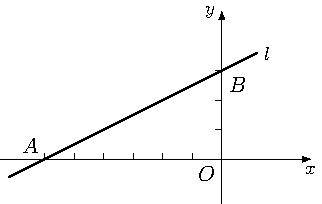
\includegraphics{1-23.pdf}
  \caption{}\label{fig:1-23}
\end{figurehere}
\end{minipage}

\medskip
画一条直线时,只要找出这条直线上的任意两点就可以了。通常是找出直线与两个坐标轴的交点。上面已经求得直线 \(l\) 与 \(x\) 轴、 \(y\) 轴的交点:
\[A\,(-6,0),\quad B\,(0,3).\]
过点 $A$、$B$ 作直线,就得直线 $l$(如\cref{fig:1-23})。

\begin{Practice}
  \begin{question}
    \item 由下列各条件,写出直线的方程,并且化成一般式:
    \begin{tasks}
      \task 斜率是 $-\dfrac{1}{2}$,经过点 $A\,(8,-2)$;
      \task 经过点 $B\,(4,2)$,平行于 $x$ 轴;
      \task 经过点 $C\,(-\dfrac{1}{2},0)$,平行于 $y$ 轴;
      \task 在 $x$ 轴和 $y$ 轴上的截距分别是 $\dfrac{3}{2}$、$-3$;
      \task 经过两点 $P_1\,(3,-2)$、$P_2\,(5,- 4)$;
      \task $x$ 轴上的截距是 $-7$,倾斜角是 \ang{45}。
    \end{tasks}
    \item 已知直线 $Ax+By+C=0$,
    \begin{tasks}
      \task 当 $B\neq 0$ 时,斜率是多少? 当 $B = 0$ 时呢?
      \task 系数为什么值时,方程表示通过坐标原点的直线。
    \end{tasks}
    \item 求下列直线的斜率和在 $y$ 轴上的截距,并画出图形:
    \begin{tasks}(3)
      \task $3x+y-5=0$;
      \task $\dfrac{x}{4}-\dfrac{y}{5}=1$;
      \task $x+2y= 0$;
      \task $7x-6y+4=0$;
      \task $2y-7= 0$。
    \end{tasks}
  \end{question}
\end{Practice}

\subsection{二元一次不等式表示的区域}
前面,我们研究了二元一次方程和直线的关系,用同样的方法,也可以研究二元一次不等式和以它的解为坐标的点的集合(图形)的关系。

含有两个未知数,并且未知数的次数都是一次的不等式叫做二元一次不等式。
使不等式成立的未知数的值叫做它的解。

我们研究不等式
\begin{equation}
  \label{eq:inequality}
  y > 2x + 1
\end{equation}
的解,并把它在坐标平面上表示出来。

\medskip\noindent
\begin{minipage}{0.65\linewidth}\parindent2em
  为了求\cref{eq:inequality} 的任何一个实数解,可任意选取 $x$ 的一个实数值,例如 $x=1$,把它看作一次方程,这个方程的图形是平行于 $y$ 轴的直线,它与直线 $l:y=2x+ 1$ 相交于点 $A\,(1,3)$(\cref{fig:1-24})。

  在直线 $x=1$ 上,点 $A$ 上方的所有点,如 $B\,(1,4)$、$C\,(1,5)$ 、……的坐标都满足\cref{eq:inequality},它们都是\cref{eq:inequality} 的解。
  
  在直线 $x=1$ 上,点 $A$ 下方的所有点,如 $B'\,(1,2)$、$C'\,(1,1)$ 、……的坐标都不满足\cref{eq:inequality},它们都不是\cref{eq:inequality} 的解。
\end{minipage}\hfill
\begin{minipage}{0.3\linewidth}\centering
\begin{figurehere}
  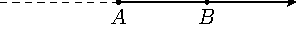
\includegraphics{1-24.pdf}
  \caption{}\label{fig:1-24}
\end{figurehere}
\end{minipage}

\medskip
可见,以\cref{eq:inequality} 的解为坐标的所有点的集合
\[P=\{M|y>2x+1\}\]
是直线 $l$ 上方的半平面所有的点,也就是\cref{fig:1-24} 中阴影所表示的平面部分,但不包括边界直线。
这种情况,直线 $l$ 在图中一般画成虚线。

以二元一次不等式的解为坐标的所有点的集合表示一个平面图形,我们把这个图形叫做不等式表示的区域。

由上例知道,$y>2x+1$ 表示的区域是直线 $l$ 上方的半平面;同理,容易求得 $y<2x+1$ 表示的区域是直线 $l$ 下方的半平面;而 $y=2x+1$ 就是边界直线 $l$。

一般地,$y=kx+b$ 的直线把平面分成两个半平面,$y>kx+b$ 表示的区域是直线上方的半平面;$y<kx+b$ 表示的区域是直线下方的半平面;直线 $y=kx+b$ 是两个半平面的边界线。

\begin{example}
  画出不等式 $y\leqslant-2x+3$ 表示的区域。
\end{example}
\begin{solution}
  不等式 $y\leqslant-2x+3$ 的解集是
  \begin{align}
    \label{eq:equality_part}   y & = -2x+3\\
    \label{eq:inequality_part} y & < -2x+3
  \end{align}
  的解集的并集,所以它们表示的区域是由\cref{eq:equality_part,eq:inequality_part} 的图形合成的。

\medskip\noindent
\begin{minipage}{0.65\linewidth}\parindent2em
  因为\cref{eq:equality_part} 的图形是直线 $l$;(2) 式的图形是直线 $l$ 下方的半平面。
  所以已知不等式表示的区域是直线 $l$ 和它下方的半平面,也就是\cref{fig:1-25} 阴影部分并且包括直线。
  这种情况,直线 $l$ 在图中一般画成实线。

  由上面的讨论容易想到,一般二元一次不等式
\[ Ax+By+C=0\]
表示的区域,一定是在直线 $Ax+By+C=0$ 的某一侧。
但要断定究竟是在哪一侧,并不需要将不等式化为 
\end{minipage}\hfill
\begin{minipage}{0.3\linewidth}\centering
  \begin{figurehere}
    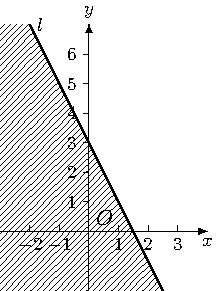
\includegraphics{1-25.pdf}
    \caption{}\label{fig:1-25}
  \end{figurehere}
\end{minipage}

\medskip\noindent
$y$ 的函数式,可以取直线 $Ax+By+C=0$ 一侧的一点,将它的坐标代入不等式,如果不等式成立,那么这一侧就是不等式表示的区域;如果不等式不成立,那么直线的另一侧是不等式表示的区域。

除选点代入不等式的方法外,也可以用 $y$ 的系数判断不等式表示的区域。如果 $B>0$ (或 $B<0$),那么不等式 $Ax+By+C>0$ 所表示的区域是直线 $Ax+By+C=0$ 的上(或下) 方的半平面;如果不等式写成  $Ax+By+C<0$ 的形式时,它表示的区域是直线下(或上)方的半平面。想一想,如果 $B=0$ 时,原不等式表示什么样的区域。
\end{solution}

\begin{example}\label{exp:1-13}
  求不等式
  \begin{equation} 
    \label{eq:inequality_2}
    x+2y-10<0
  \end{equation}
  表示的区域,并画出图形。
\end{example}
\noindent
\begin{minipage}{0.45\linewidth}\parindent2em
\begin{solution}
  先画出直线 $l:x+2y-10=0$。

  用选点代入\cref{eq:inequality_2} 的方法,例如将原点 $(0,0)$ 的坐标代入\cref{eq:inequality_2},得 $-10<0$,\cref{eq:inequality_2} 成立。
  所以坐标原点所在的半平面是\cref{eq:inequality_2} 表示的区域,即直线 $l$ 下方的半平面,如\cref{fig:1-26} 的阴影部分,但不包括直线 $l$。
\end{solution}
\end{minipage}\hfill
\begin{minipage}{0.5\linewidth}
\begin{figurehere}
  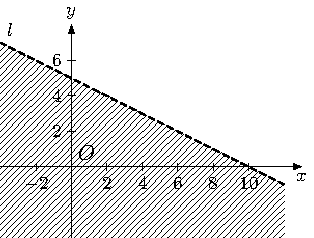
\includegraphics{1-26.pdf}
  \caption{}\label{fig:1-26}
\end{figurehere}
\end{minipage}

\medskip
\cref{exp:1-13} 也可以用如下解法:

\begin{solution}
  用 $y$ 的系数判断\cref{eq:inequality_2} 表示的区域。

  $\because \; B=2>0$,
  
  $\therefore\; x+2y-10<0$ 表示的区域是直线 $x+2y-10=0$ 下方的半平面,但不包括直线。
\end{solution}

\begin{example}
  某工厂有一批长为 \qty{2.5}{m} 的条形钢材,要截成 \qty{60}{cm} 和 \qty{42}{cm} 两种规格的零件毛坯,找出最佳的下料方案并计算材料的利用率。
\end{example}
\noindent
\begin{minipage}{0.58\linewidth}\parindent2em
\begin{solution}
  设每根钢材可截成 \qty{60}{cm} 长的毛坯 $x$ 根和 \qty{42}{cm} 长的毛坯 $y$ 根。按题意得不等式
  \begin{equation}
    \label{eq:inequality_3}
    0.6x+0.42y\leqslant 2.5
  \end{equation}

  在坐标纸上画出
  \begin{equation}
    \label{eq:equality_3}
    0.6x+0.42y= 2.5
  \end{equation}
  的直线。如\cref{fig:1-27}。

  因为要截得的两种毛坯数的和必须是正整数,所以以\cref{eq:inequality_3} 的解为坐标的点一定是第一象限内的网格的交点。
\end{solution}
\end{minipage}\hfill
\begin{minipage}{0.37\linewidth}\centering
\begin{figurehere}
  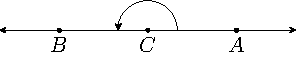
\includegraphics{1-27.pdf}
  \caption{}\label{fig:1-27}
\end{figurehere}
\end{minipage}

\medskip
如果直线~\eqref{eq:equality_3} 上有网格的交点,那么按直线上网格交点的坐标 $(x,y)$ 的值作为下料方案,这时材料全被利用,因此这个方案就是最佳方案。
但从\cref{fig:1-27}中可以看出,直线~\eqref{eq:equality_3} 不通过网格交点,在这种情况下,为了制订最佳下料方案,应该找靠近直线~\eqref{eq:equality_3} 的网格交点。

当然不能在直线~\eqref{eq:equality_3} 的上方半平面内找网格交点。
因为 $B=0.42>0$,上方半平面内任何网格交点的坐标都使 $0.6x+0.42y>2.5$,这时两种零件毛坯长度的和超过了原钢材长,这是不合理的。

这样,下料范围只能限制在 $0.6x+0.42y<2.5$ 表示的区域内。这个区域是直线~\eqref{eq:equality_3} 下方的半平面。
在直线~\eqref{eq:equality_3} 的下方半平面上找到最靠近直线的网格交点,得点 $M\,(2,3)$。

$x=2$,$y=3$ 就是所求的解,按这样截取毛坯,材料尽管没有被完全利用,但废料最少。

材料的利用率
\[ \frac{0.6 \times 2 + 0.42 \times 3}{2.5} =98.4\%.\]
答: 把每根条钢截成 2 根 \qty{60}{cm} 长和 3 根 \qty{42}{cm} 长的零件毛坯是最佳的下料方案。材料利用率为 98.4\%。

\begin{Practice}
  \begin{question}
    \item 求下列不等式表示的区域:
    \begin{tasks}(3)
      \task $y<-2x-1$;
      \task $y\geqslant -x+3$;
      \task $x+2y-15<0$;
      \task $5x-3y+2\leqslant o$;
      \task $x\geqslant 4$;
      \task $y\leqslant -3$;
      \task $y\leqslant 3x$;
      \task $x\leqslant -2y$;
      \task $3x+2y<0$。
    \end{tasks}
    \item 已知 $y<kx+b$ 表示直线 $y=kx+b$ 下方的半平面,说明当 $B<0$ 时,不等式 $Ax+By+C>0$ 表示的区域是直线 $Ax+By+C=0$ 下方的半平面。
    \item 已知每袋面粉 \qty{25}{kg},每袋大米 \qty{105}{kg},用栽重量是 \qty{265}{kg} 的小推车运输,找出车运效率最高的装车方案。
  \end{question}
\end{Practice}

\subsection{直线型经验公式}
在生产和科学实验中,常常需要根据观察或实验所得的两个变量的一些对应的近似值(叫做实验数据),来求出这两个变量之间的函数关系的解析式。
这样通过实验数据得到的两个变量的关系式叫做经验公式。
如果所求得的经验公式是一次方程,它就叫做直线型经验公式。

下面举例说明求直线型经验公式的方法。
\begin{example}
  通过实验,测得某种合金的熔点 $y$(\unit{\celsius})和含铅量 $x$(\%)之间关系的数据如\cref{tab:1-1}:
  \begin{table}
    \caption{某种合金的熔点 $y$(\unit{\celsius})和含铅量 $x$(\%)之间关系}\label{tab:1-1}
    \begin{tblr}{colspec={X[c]*6{X[r]}},vline{2}=0.8pt}
      $x$(\%)              & 36.9 & 46.7 & 63.7 & 77.8 & 84.0 & 87.5 \\
      $y$(\unit{\celsius}) & 181  & 197  & 235  & 270  & 283  & 292  \\
    \end{tblr}
  \end{table}
  根据这些数据,求关于 $x$、$y$ 的经验公式。
\end{example}
\noindent
\begin{minipage}{0.45\linewidth}\parindent2em
\begin{solution}
  \begin{enumerate}
    \item 把各组对应的数据作为点的坐标,在坐标平面上画出这些点。
    例如,以 $(63.7,235)$ 为坐标的点就是 $P$(\cref{fig:1-28})。
    \item 观察这些点的位置,可以看出它们大致分布在一条直线上。
    用透明尺的边缘在这些点间移动,使它尽量靠近或通过大多数点,然后画出直线。
    \item 求方程:在这条直线上选出两点,例如 $A\,(46.7,197)$、$B\,(84.0,283)$。
    把它们的坐标代入直线的两点式方程,得
    \[ \frac{y-197}{283-197}=\frac{x-46.7}{84.0-46.7}\]
    化简后,就得经验公式
    \[ y=2.3x+89.3\]
  \end{enumerate}
\end{solution}
\end{minipage}\hfill
\begin{minipage}{0.5\linewidth}\centering
\begin{figurehere}
  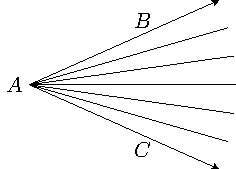
\includegraphics{1-28.pdf}
  \caption{}\label{fig:1-28}
\end{figurehere}
\end{minipage}

\medskip
有了这个经验公式,就可以从这种合金的含铅量求得对应的熔点,或者反过来,从这种合金的熔点求得对应的含铅量。

上面这种选择两点求直线型经验公式的方法,叫做\Concept{选点法}。

选点法虽然比较简便,但是由于选点的灵活性较大,一般精确度不高。下面再介绍一种精确度较高的方法,叫做\Concept{平均值法}。

我们仍用上面的例题来说明平均值法。
在确定经验公式是直线型的以后,可假定所求的经验公式为
\[y=kx+b\]

把表中 $x$、$y$ 的对应值代入这个方程,得到若干个关于 $k$、 $b$ 的一次方程。
为了确定 $k$、$b$ 的值,把它们分成两组,使两组中的方程个数相同或相差一个,再把各组方程两边分别相加,就得到关于 $k$、$b$ 的两个方程:
\[ 
  \begin{array}{rcrcr}
      181 &=& 36.9k&+&b \\
      197 &=& 46.7k&+&b \\
   +)\quad 235 &=& 63.7k&+&b \\
   \hline 
    613 &=& 147.3k&{}+&3b 
  \end{array}\qquad 
  \begin{array}{rcrcr}
    270 &=& 77.8k&+&b \\
    283 &=& 84.0k&+&b \\
 +)\quad 292 &=& 87.5k&+&b \\
 \hline 
  845 &=& 249.3k&{}+&3b 
\end{array}
\]
解方程组
\[ \begin{cases} 
  613=147.3k+3b,\\
  845=249.3+3b,
\end{cases}\]
得
\[ k\approx 2.27,\quad b\approx 92.9.\]

代入所设方程,就得到所求的经验公式
\[ y=2.27b+92.9.\]

\begin{Practice}
  \begin{question}
    \item 丙烯腈是合成人造羊毛的原料。在研究它的比重 $D$ 和温度 $T$(\unit{\celsius})的关系时,通过实验得到的数据如下:\par\noindent
    \begin{tablehere}
    \begin{tblr}{colspec={c*{7}{X[c]}},vline{2}=0.8pt}
      $T$(\unit{\celsius})& 0 & 5 & 10 & 15 & 20 & 25 & 30 \\
      $D$                   & 0.8287 &0.8282 & 0.8276 & 0.8271 &0.8266 & 0.8261& 0.8255 \\
    \end{tblr}
  \end{tablehere}
    用选点法求出 $D$ 与 $T$ 之间的经验公式。
    \item 根据下列实验数据,用平均值法求关于 $m$、$p$ 的经验公式:\par\noindent
    \begin{tablehere}
      \begin{tblr}{colspec={*{8}{X[c]}},vline{2}=0.8pt}
        $m$ & 0.03 & 0.06 & 0.10 & 0.14 & 0.17 & 0.20 & 0.25 \\
        $p$ & 0 & 0.42 & 0.93 & 1.60 & 2.03 & 2.41 & 3.31 \\
      \end{tblr}
    \end{tablehere}
  \end{question}
\end{Practice}

\begin{Exercise}
  \begin{question}
    \item 四边形 $ABCD$ 的四个顶点是 $A\,(2,3)$、$B\,(1,-1)$、$C\,(-1,-2)$、$D\,(-2,2)$。求四边所在直线的倾斜角和斜率。
    \item 根据下列条件写出直线的方程:
    \begin{tasks}
      \task 斜率是 $\dfrac{\sqrt{3}}{3}$,经过点 $A\,(8,-2)$;
      \task 过点 $B\,(-2,0)$,且与 $x$ 轴垂直;
      \task 斜率为 $-4$,在  $y$ 轴上的截距为 7;
      \task 经过两点 $A\,(-1,8)$、$B\,(4,-2)$;
      \task 在 $y$ 轴上的截距是 2,且与 $x$ 轴平行;
      \task 在 $x$ 轴、$y$ 轴上的截距分别是 4 与 $-3$。
    \end{tasks}
    \item 已知直线的斜率 $k=2$,$P_1\,(3,5)$、$P_2\,(x_2,7)$、$P_3\,(-1,y_3)$ 是这条直线上的三个点。求 $x_2$ 和 $y_3$。
    \item 已知两点 $M\,(2,2)$ 和 $N\,(5,-2)$,点 $P$ 在 $x$ 轴上,且 $\angle MPN =\ang{90}$。求点 $P$ 的坐标。
    \item 设 $A$、$B$ 两点的坐标分别是 $(x_1,y_1)$ 和 $(x_2,y_2)$,直线 $AB$ 的倾斜角是 $\alpha$。求证:
    \[|x_1-x_2|=\sqrt{(x_2-x_1)^2+(y_2-y_1)^2}|\cos\alpha|\]
    \item 一条直线经过点 $A\,(2,-3)$,它的倾斜角等于直线 $y=\dfrac{1}{\sqrt{3}}x$ 的倾斜角的 2 倍,求这条直线的方程。
    \item 一根弹簧,挂 \qty{4}{kg} 的物体时,长 \qty{20}{cm},在弹性限度内,所挂物体的重量每增加 \qty{1}{kg},弹簧伸长 \qty{1.5}{cm}。利用点斜式写出弹簧的长度 $l$(\unit{cm})和所挂物体重量 $F$(\unit{kg})之间关系的方程。
    \item 一条直线和 $y$ 轴相交于点 $P\,(0,2)$,它的倾斜角的正弦是 $\dfrac{4}{5}$。求这条直线的方程。这样的直线有几条?
    \item 证明:三点 $A\,(1,3)$、$B\,(5,7)$、$P\,(10,12)$ 在同一条直线上。
    \item 解答:
    \begin{tasks}
      \task 已知三角形的顶点是 $A\,(8,5)$、$B\,(4,-2)$、$C\,(-6,3)$,求经过每两边中点的三条直线的方程。
      \task $\triangle ABC$ 的顶点是 $A\,(0,5)$、$B\,(1,-2)$、$C\,(-6,4)$,求 $BC$ 边上的中线所在直线的方程。
    \end{tasks}
    \item 一根铁棒在 \qty{40}{\celsius} 时长 \qty{12.506}{m},在 \qty{80}{\celsius} 时长 \qty{12.512}{m},已知长度 $l$(\unit{m})和温度 $t$(\unit{\celsius})的关系可以用直线方程来表示,用两点式表示这个方程,并且根据这个方程,求这根铁棒在 \qty{100}{\celsius} 时的长度。
    \item 菱形的两条对角线长分别等于 8 和 6,并且分别放置在 $x$ 轴和 $y$ 轴上。求菱形各边所在的直线的方程。
    \item 求过点 $P\,(2,3)$,并且在两轴上的截距相等的直线方程。
    \item 油槽储油 \qty{20}{m^3},从一管道等速流出,\qty{50}{min} 流完。用截距式写出关于油槽里剩余的油量 $Q$(\unit{m^3})和流出的时间 $t$(\unit{min})的方程,并且画出图形(注意: $0\leqslant t \leqslant 50$)。
    \item 直线方程 $Ax+By+C=0$ 的系数 $A$、$B$、$C$ 满足什么关系时,这条直线
    \begin{tasks}(3)
      \task 与坐标轴都相交;
      \task 只与 $x$ 轴相交;
      \task 只与 $y$ 轴相交;
      \task 是 $x$ 轴;
      \task 是 $y$ 轴。
    \end{tasks}
    \item 设点 $P\,(x_0,y_0)$ 在直线 $Ax+By+C=0$ 上。求证:这条直线的方程可以写成 $A(x-x_0)+B(y-y_0)=0$。
    \item 求下列不等式表示的区域:
    \begin{tasks}(3)
      \task $y \geqslant x$;
      \task $x<2y$;
      \task $3y \leqslant 2x$;
      \task $3y-2 \leqslant 0$;
      \task $3x-5y+10>0$;
      \task $2x+3y-4 \geqslant 0$。
    \end{tasks}
    \item 某同学拿 5 元钱买纪念邮票,票面 4 分钱的每套 5 张,8 分钱的每套 4 张。如果每种至少买一套,共有几种买法,能否恰好将钱用完,怎样买剩钱最少?
    \item 有一滑轮组,举起的物重 \(W\) 与需用的力 \(F\) 之间的关系,由实验所得的数据如下表:
    \begin{tablehere}
      \begin{tblr}{colspec={*6{X[c]}},vline{2}={0.8pt}}
        $W$(\unit{kg}) & 20 & 40 & 60 & 80 & 100 \\
        $F$(\unit{kgf})& 4.35 & 7.55 & 10.40 & 13.80 & 16.80 \\
      \end{tblr}
    \end{tablehere}
    求适合以上关系的直线型经验公式。
    \item 一个弹簧的长度 $l$ 和它悬挂的重量 $W$ 间关系的实验数据如下:
    \begin{tablehere}
      \begin{tblr}{colspec={*7{X[c]}},vline{2}={0.8pt}}
        $W$ & 2 & 4 & 6 & 8 & 10 & 12 \\
        $l$ & 8.9 & 10.1 & 11.2 & 12.0 & 13.1 & 13.9 \\
      \end{tblr}
    \end{tablehere}
    分别用选点法和平均值法求关于 $l$、$W$ 的经验公式,并算出当 $l=9.2$ 时,$W$ 的值。
  \end{question}
\end{Exercise}

\section{两条直线的位置关系}
\subsection{两条直线的平行与垂直}
在平面几何中,我们研究过平面上两条直线互相平行或垂直的位置关系。
现在我们研究怎样通过直线的方程来判定两条直线平行或垂直。

设直线 $l_1$ 和 $l_2$ 的斜率为 $k_1$ 和 $k_2$,它们的方程分别是
\[ l_1:y =k_1x+b_1;\quad l_2:y =k_2x+b_2. \]

我们首先研究两条直线平行(不重合)的情形。

\medskip\noindent
\begin{minipage}{0.6\linewidth}\parindent2em
如果 $l_1\parallel l_2$(\cref{fig:1-29}),那么它们的倾斜角相等,$\alpha_1=\alpha_2$。

$\therefore \quad \tan\alpha_1=\tan\alpha_2$,即 $k_1=k_2$。

反过来,如果两条直线的斜率相等,$k_1=k_2$,也就是 $\tan\alpha_1=\tan\alpha_2$。

由于 $\ang{0}\leqslant\alpha_1<\ang{180}$,$\ang{0}\leqslant\alpha_2<\ang{180}$,

$\therefore \quad \tan\alpha_1=\tan\alpha_2$。

又因为两条直线不重合,

$\therefore l_1\parallel l_2$。
\end{minipage}\hfill
\begin{minipage}{0.35\linewidth}\centering
\begin{figurehere}
  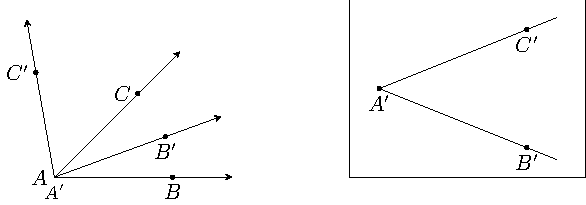
\includegraphics{1-29.pdf}
  \caption{}\label{fig:1-29}
\end{figurehere}
\end{minipage}

\bigskip
两条直线有斜率且不重合,如果它们平行,则斜率相等;反之,如果它们的斜率相等,则它们平行。即
\[ \tcbhighmath{l_1\parallel l_2 \Leftrightarrow k_1=k_2}.\]
\begin{example}
  已知两条不重合的直线
  \[ l_1:2x-4y+7=0,\quad l_2:x-2y+5=0. \]
  求证:$l_1\parallel l_2$。
\end{example}
\begin{proof}
  把 $l_1$、$l_2$ 的方程写成斜截式:
  \[ l_1:y=\frac{1}{2}x+\frac{7}{4},\quad l_2:y=\frac{1}{2}x+\frac{5}{2}. \]
  则 $l_1$ 的斜率 $k_1=\dfrac{1}{2}$,$l_2$ 的斜率 $k_1=\dfrac{1}{2}$,
  
  $\therefore\quad k_1=k_2.$

  又 $\because$ 两条直线不重合,

  $\therefore\quad l_1\parallel l_2.$
\end{proof}

\begin{example}
  求过点 $A\,(1,- 4)$,且与直线 $2x+3y+5=0$ 平行的直线方程。
\end{example}

\begin{solution}
已知直线的斜率是 $-\dfrac{2}{3}$,因为所求直线与已知直线平行,因此它的斜率也是 $-\dfrac{2}{3}$。

根据点斜式,得到所求直线的方程是
\[ y+4=-\frac{2}{3}(x-1),\]
即
\[ 2x+3y+10=0.\]
\end{solution}

现在研究两条直线垂直的情形。

如果 \(l_1 \perp l_2\) ,这时 $\alpha_1\neq\alpha_2$,(为什么?)

设 $\alpha_2<\alpha_1$(\cref{fig:1-30})。
根据三角形外角等于和它不相邻的两内角的和,得
\[ \alpha_1=\ang{90}+\alpha_2. \]
\begin{figure}
  \begin{minipage}[b]{0.48\linewidth}\centering
  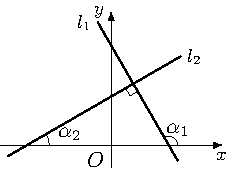
\includegraphics{1-30a.pdf}
  \subcaption{}\label{fig:1-30a}
  \end{minipage}
  \begin{minipage}[b]{0.48\linewidth}\centering
  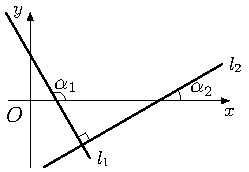
\includegraphics{1-30b.pdf}
  \subcaption{}\label{fig:1-30b}
  \end{minipage}
  \caption{}\label{fig:1-30}
\end{figure}

因为 $l_1$、$l_2$ 的斜率是 $k_1$、$k_2$,即 $\alpha_1\neq\ang{90}$,所以 $\alpha_2\neq\ang{0}$。
\[ \therefore \tan\alpha_1 = \tan(\ang{90}+\alpha_2) = - \frac{1}{\tan\alpha_2} \]
即
\[
k_1=-\frac{1}{k_2}\;\text{ 或 }\;k_1 \cdot k_2 = -1.
\]

反过来,如果 $k_1=-\dfrac{1}{k_2}$,即 $k_1 \cdot k_2 = -1$。设其中一个,例如 $k_2$ 是正数,则 $k_1$ 是负数。
那么 $\alpha_2$ 是锐角,$\alpha_1$ 是钝角。于是由
\[ \tan\alpha_1 = - \frac{1}{\tan\alpha_2} = \tan(\ang{90}+\alpha_2), \]
可以推出
\begin{gather*}
  \alpha_1 = \ang{90} + \alpha_2,\\
l_1 \perp l_2.
\end{gather*}

两条直线都有斜率,如果它们互相垂直,则它们的斜率互为负倒数;反之,如果它们的斜率互为负倒数,则它们互相垂直。即
\[ \tcbhighmath{l_1 \perp l_2 \Leftrightarrow k_1=-\frac{1}{k_2}}. \]
或 $ l_1 \perp l_2 \Leftrightarrow k_1 \cdot k_2 = -1$。

\begin{example}
已知两条直线
\[l_1:2x-4y+7=0, \quad l_2:2x+y-5=0\]
求证:$l_1\perp l_2$
\end{example}
\begin{proof}
$l_1$ 的斜率 $k_1=\dfrac{1}{2}$,$l_2$ 的斜率 $k_2=-2$。

由于 $k_1\cdot k_2 =\dfrac{1}{2}\times(-2)=-1$,

$\therefore \quad l_1\perp l_2$。
\end{proof}

\begin{example}
求过点 $A\,(2,1)$,且与直线 $2x+y-10=0$ 垂直的直线方程。
\end{example}

\begin{solution}
  直线 $2x+y-10=0$ 的斜率是 $-2$。因为所求直线与已知直线垂直,所以它的斜率
  \[ k= -\frac{1}{-2}=\frac{1}{2}.\]

  根据点斜式,得到所求直线的方程是
\[ y-1=\frac{1}{2}(x-2), \]
就是
\[ x-2y= 0. \]
\end{solution}

\begin{Practice}
  \begin{question}
    \item 判别下列各对不重合的直线是否平行或垂直:
    \begin{tasks}(2)
      \task $y=3x+4$ 与 $2y-6x+1=0$;
      \task $y=x$ 与 $3x+3y-10=0$;
      \task $3x+4y=5$ 与 $6x-8y=7$;
      \task! $\sqrt{3}x-y-1=0$ 与 $\sqrt{3}x+3y+6=0$。
    \end{tasks}
    \item 求过点 $A\,(2,3)$,且分别适合下列条件的直线方程:
    \begin{tasks}(2)
      \task 平行于直线 $2x+y-5=0$;
      \task 垂直于直线 $x-y-2=0$。
    \end{tasks}
    \item 已知两条直线 $l_1$、$l_2$,其中一条没有斜率。这两条直线什么时候
    \begin{tasks}(2)
      \task 平行;
      \task 垂直。
    \end{tasks}
    逆命题成立吗?
  \end{question}
\end{Practice}

\subsection{两条直线所成的角}
\medskip\noindent
\begin{minipage}{0.7\linewidth}\parindent2em
两条直线 $l_1$ 和 $l_2$ 相交构成四个角,它们是两对对顶角。
为了区别这些角,我们把直线 $l_1$ 依逆时针方向旋转到与 $l_2$ 重合时所转的角,叫做 \Concept{$l_1$ 到 $l_2$ 的角},\cref{fig:1-31} 中,直线 $l_1$ 到 $l_2$ 的角是 $\theta_1$,$l_2$ 到 $l_1$ 的角是 $\theta_2$($\theta_1+\theta_2=\ang{180}$)。
\end{minipage}\hfill
\begin{minipage}{0.25\linewidth}\centering
\begin{figurehere}
  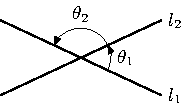
\includegraphics{1-31.pdf}
  \caption{}\label{fig:1-31}
\end{figurehere}
\end{minipage}

\medskip
现在我们来求斜率为 $k_1$、$k_2$ 的两条直线 $l_1$ 到 $l_2$ 的角 $\theta$。设已知直线的方程分别是
\begin{gather*}
  l_1: y=k_1x+b_1,\\
  l_2: y=k_2x+b_2.
\end{gather*}

如果 $1+k_1k_2=0$,那么 $\theta = \ang{90}$。

下面研究 $1+k_1k_2\neq0$ 的情形。

设 $l_1$、$l_2$ 的倾斜角分别是 $\alpha_1$ 和 $\alpha_2$(\cref{fig:1-32}),
\[ \tan\alpha_1=k_1,\quad \tan\alpha_2=k_2.\]
\begin{figure}
  \begin{minipage}[b]{0.48\linewidth}\centering
  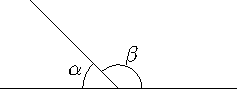
\includegraphics{1-32a.pdf}
  \subcaption{}\label{fig:1-32a}
  \end{minipage}
  \begin{minipage}[b]{0.48\linewidth}\centering
  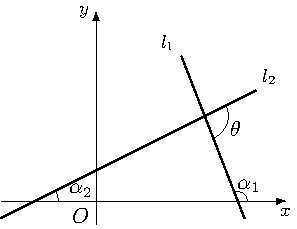
\includegraphics{1-32b.pdf}
  \subcaption{}\label{fig:1-32b}
  \end{minipage}
  \caption{}\label{fig:1-32}
\end{figure}

$\because\quad\theta =\alpha_2-\alpha_1$(\cref{fig:1-32a})或 $\theta = \uppi - (\alpha_1-\alpha_2) = \uppi+(\alpha_2-\alpha_1)$(\cref{fig:1-32b}),

$\therefore\quad\tan\theta = \tan(\alpha_2-\alpha_1)$ 或 $\tan\theta = \tan[\uppi+(\alpha_2-\alpha_1)]= \tan(\alpha_2-\alpha_1)$。可得
\[ \tan\theta=\frac{\tan\alpha_2-\tan\alpha_1}{1+\tan\alpha_2\tan\alpha_1},\]
即
\[ \tan\theta = \frac{k_2-k_1}{1+k_2k_1}.\]

从一条直线到另一条直线的角,可能不大于直角,也可能大于直角,但我们常常只需要考虑不大于直角的角(就是两条直线所成的角,简称\Concept{夹角})就可以了,这时可用下面的公式
\[ \tcbhighmath{\tan\theta = \left|\frac{k_2-k_1}{1+k_2k_1}\right|}.\]

\begin{example}
  求直线 $l_1:y=-2x+3$,$l_2:y=x-\dfrac{3}{2}$ 的夹角。
\end{example}
\begin{solution}
  两条直线的斜率为 $k_1= -2$,$k_2=1$,得
  \begin{gather*}
  \tan \theta = \left|\frac{k_2-k_1}{1+k_2k_1}\right| =\left|\frac{1-(-2)}{1+1\cdot(-2)k}\right|=3.\\
  \therefore\quad \theta=\arctan3\approx\ang{71;34;}.
  \end{gather*}
\end{solution}
\begin{example}
  求直线 $l_1:A_1x+B_1y+C_1=0$ 和 $l_2:A_2x+B_2y+C_2=0$($B_1\neq 0$、$B_2\neq 0$、$A_1A_2+B_1B_2\neq 0$),$l_1$ 到 $l_2$ 的角是 $\theta$。
  求证:
  \[ \tan\theta = \frac{A_1B_2-A_2B_1}{A_1A_2+B_1B_2}.\]
\end{example}
\begin{proof}
  设两条直线 $l_1$、$l_2$ 的斜率分别为 $k_1$、$k_2$,则
  \begin{gather*}
    k_1=-\frac{A_1}{B_1},\quad k_2=-\frac{A_2}{B_2},\\
    \therefore\quad \tan\theta=\frac{k_2-k_1}{1+k_2k_1}=\frac{-\dfrac{A_2}{B_2}-\left(-\dfrac{A_1}{B_1}\right)}{1+\left(-\dfrac{A_2}{B_2}\right)\left(-\dfrac{A_1}{B_1}\right)}=\frac{A_1B_2-A_2B_1}{A_1A_2+B_1B_2}.
  \end{gather*}
\end{proof}

\begin{example}
  等腰三角形一腰所在的直线 $l_1$ 的方程是 $x-2y-2=0$,底边所在的直线 $l_2$ 的方程是 $x+y-1=0$,点 $(-2,0)$ 在另一腰上,求这腰所在直线 $l_3$ 的方程。
\end{example}
\begin{solution}
  设 $l_1$、$l_2$、$l_3$ 的斜率分别为 $k_1$、$k_2$、$k_3$,$l_1$ 到 $l_2$ 的角是 $\theta_1$,$l_2$ 到 $l_3$ 的角是 $\theta_2$。则
  \begin{gather*} 
    k_1=\frac{1}{2},\quad k_2=-1,\\
    \tan\theta_1=\frac{k_2-k_1}{1+k_2k_1}=\frac{(-1)-\dfrac{1}{2}}{1+(-1)\cdot\dfrac{1}{2}}=-3.
  \end{gather*}
  因为 $l_1$、$l_2$、$l_3$ 所围成的三角形是等腰三角形,所以
  \begin{gather*} 
    \theta_1=\theta_2,\\
    \tan\theta_2=\tan\theta_2=-3.
  \end{gather*}
  即
  \begin{gather*} 
    \frac{k_3-k_2}{1+k_3k_2}=-3.\\
    \frac{k_3+1}{1-k_3}=-3.
  \end{gather*}
  解得
  \[ k_3=2.\]

  因为 $l_3$ 经过点 $(-2,0)$,斜率为 2,写出点斜式为
  \[ y=2[x-(-2)],\]
  得
  \[ 2x-y+4=0.\]

  这就是直线 $l_3$ 的方程。
\end{solution}

\begin{Practice}
  \begin{question}
    \item 求下列直线 $l_1$ 到 $l_2$ 的角与 $l_2$ 到 $l_1$ 的角:
    \begin{tasks}
      \task $l_1: y=\dfrac{1}{2}x+2,\quad l_2:y=3x+7$;
      \task $l_1: x-y=5,\quad l_2: x+2y-3=0$。
    \end{tasks}
    \item 求下列直线的夹角:
    \begin{tasks}(2)
      \task $y=3x-1,\quad y=-\dfrac{1}{3}x+4$;
      \task $x-y=5, \quad y=4$;
      \task $5x-3y=9, 6x+10y+7=0$。
    \end{tasks}
  \end{question}
\end{Practice}

\subsection{两条直线的交点}
设两条直线的方程是
\[l_1:A_1x+B_1y+C_1=0,\quad l_2:A_2x+B_2y+C_2=0.\]

如果这两条直线相交,由于交点同时在这两条直线上,交点的坐标一定是这两个方程的公共解;反之,如果这两个二元一次方程只有一个公共解,那么以这个解为坐标的点必是直线 $l_1$ 和 $l_1$ 的交点。
因此,两条直线是否有交点,就要看这两条直线的方程所组成的方程组
\begin{numcases}{}
  \label{eq:line_eq_1} A_1x+B_1y+C_1=0 \\ 
  \label{eq:line_eq_2} A_2x+B_2y+C_2=0  
\end{numcases}
是否有唯一解。

设 $A_1$、$A_2$、$B_1$、$B_2$ 全不为零。

解这个方程组,
\begin{align}
  \label{eq:eq1_times_B2} \text{\eqref{eq:line_eq_1}} \times B_2\ \text{得}\quad A_1B_2x+B_1B_2y+B_2C_1=0 \\
  \label{eq:eq2_times_B1} \text{\eqref{eq:line_eq_2}} \times B_1\ \text{得}\quad A_2B_1x+B_1B_2y+B_1C_2=0 
\end{align}

\cref{eq:eq1_times_B2}$-$\cref{eq:eq2_times_B1} 得 $(A_1B_2-A_2B_1)x+B_2C_1-B_1C_2=0$。

下面分两种情形进行讨论:
\begin{enumerate}
  \item 当 $A_1B_2-A_2B_1\neq 0$ 时,即 $\dfrac{A_1}{A_2} \neq \dfrac{B_1}{B_2}$ 时,方程有唯一解:
  \[ \begin{cases}
    x=\dfrac{B_1C_2-B_2C_1}{A_1B_2-A_2B_1}\\[10pt]
    y=\dfrac{C_1A_2-C_2A_1}{A_1B_2-A_2B_1}\\
  \end{cases}\]

  这时 $l_1$ 与 $l_2$ 相交,上面 $x$ 和 $y$ 的值就是交点的坐标。

  \medskip 因为直线 \eqref{eq:line_eq_1} 和 \eqref{eq:line_eq_2} 的斜率分别是 $-\dfrac{A_1}{B_1}$ 和 $-\dfrac{A_2}{B_2}$,由 $\dfrac{A_1}{B_1} \neq \dfrac{A_2}{B_2}$ 可得 $-\dfrac{A_1}{B_1}\neq -\dfrac{A_2}{B_2}$,也就是说,两条直线的斜率不相等,它们必相交于一点。

\medskip 例如,两条直线的方程是
\begin{align*}
  2x+3y-7 & = 0,\\
  5x-y-9 & = 0.
\end{align*}

由于 $\dfrac{2}{5} \neq \dfrac{3}{-1}$,这两个方程组成的方程组有唯一解,并且这个解是
\[\begin{cases}x=2\\y=1\end{cases}\]
就是说,这两条直线相交,交点的坐标是 $(2,1)$。

  \item 当 $A_1B_2-A_2B_1= 0$ 时:
  \begin{enumerate}
    \item 如果 $B_1C_2-B_2C_1\neq 0$,这时 $C_1$、$C_2$ 不能全为零。
    设 $C_2\neq 0$,有 $\dfrac{A_1}{A_2}=\dfrac{B_1}{B_2} \neq \dfrac{C_1}{C_2}$。方程组无解,也就是说这两条直线不相交,即两直线平行。

    \medskip 因为 $\dfrac{A_1}{A_2}=\dfrac{B_1}{B_2}\neq\dfrac{C_1}{C_2}$,即 $\dfrac{A_1}{B_1}=\dfrac{A_2}{B_2}$,$\dfrac{C_1}{B_1} \neq \dfrac{C_2}{B_2}$,所以直线 \eqref{eq:line_eq_1} 和 \eqref{eq:line_eq_2} 的斜率 $-\dfrac{A_1}{B_1}=- \dfrac{A_2}{B_2}$,截距 $\dfrac{C_1}{B_1} \neq \dfrac{C_2}{B_2}$,显然两条直线平行。

    \medskip 例如,两条直线的方程是
    \begin{align*}
      2x-3y+5 & = 0,\\
      4x-6y-7 & = 0.
    \end{align*}

    因为 $\dfrac{2}{4} = \dfrac{-3}{-6} \neq \dfrac{5}{-7}$,所以方程组没有解,两条直线平行。
    \item 如果 $B_1C_2-B_2C_1\neq 0$,这时 $C_1$、$C_2$ 或全为零,或全不为零$\biggl($当 $C_1$、$C_2$ 全不为零时,$\dfrac{A_1}{A_2}= \dfrac{B_1}{B_2}=\dfrac{C_1}{C_2}\biggr)$。
    两个方程是同解方程,因此它们有无穷多解。

    \medskip 这时两条直线的斜率 $-\dfrac{A_1}{B_1}=-\dfrac{A_2}{B_2}$,在 $y$ 轴上的截距 $-\dfrac{C_1}{B_1}=-\dfrac{C_2}{B_2}$(当 $C_1$、$C_2$ 全为零时,两条直线都通过原点),两方程的直线重合。

例如,两条直线的方程是
\begin{align*}
  2x-3y+5 & = 0,\\
  4x-6y+10 & = 0.
\end{align*}
由于 $\dfrac{2}{4} = \dfrac{-3}{-6} = \dfrac{5}{10}$,两个方程是同解方程,方程组有无穷多个解,两条直线重合。
  \end{enumerate}
\end{enumerate}

\bigskip 如果 $A_1$、$A_2$、$B_1$、$B_2$ 中有等于零的情形,方程比较简单,两条直线的交点很容易讨论。
\begin{example}
  求下列两条直线的交点。
  \begin{align*}
    l_1:&&3x+4y-2 & = 0,\\
    l_2:&&2x+y+2 & = 0.
  \end{align*}
\end{example}
\noindent
\begin{minipage}{0.6\linewidth}\parindent2em
\begin{solution}
  解方程组
  \[\begin{cases} 3x+4y=0,\\2x+y+2=0. \end{cases}\]
  得
  \[\begin{cases} x=-2,\\y=2. \end{cases}\]
  $\therefore \quad l_1$ 与 $l_2$ 的交点是 $M\,(-2,2)$,如\cref{fig:1-33} 所示。
\end{solution}
\end{minipage}\hfill
\begin{minipage}{0.35\linewidth}\centering
\begin{figurehere}
  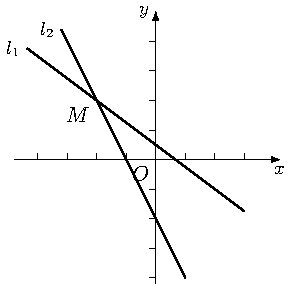
\includegraphics{1-33.pdf}
  \caption{}\label{fig:1-33}
\end{figurehere}
\end{minipage}

\medskip
\begin{example}
  已知两条直线:
  \begin{align*}
    l_1:&&x+my+6 & = 0,\\
    l_2:&&(m-2)x+3y+2m & = 0.
  \end{align*}
  当 $m$ 为何值时,${l}_{1}$ 与 ${l}_{2}$ 
  \begin{tasks}(3)
    \task 相交;
    \task 平行;
    \task 重合。
  \end{tasks}
\end{example}
\begin{solution}
  将两直线的方程组成方程组
  \[\begin{cases} x+my+6=0,\\(m-2)x+3y+2m=0. \end{cases}\]

  这时,$\dfrac{A_1}{A_2}=\dfrac{1}{m - 2}$,$\dfrac{B_1}{B_2} = \dfrac{m}{3}$,$\dfrac{C_1}{C_2} = \dfrac{6}{2m}$。

  \medskip 当 $\dfrac{A_1}{A_2}=\dfrac{B_1}{B_2}$ 时,$\dfrac{1}{m-2} = \dfrac{m}{3}$,解得 $m=-1$ 或 $m=3$。

\medskip 当 $\dfrac{A_1}{A_2}=\dfrac{C_1}{C_2}$ 时,$\dfrac{1}{m-2} = \dfrac{6}{2m}$,解得 $m=3$。
\begin{enumerate}
  \item 当 $m\neq-1$ 且 $m\neq 3$ 时,$\dfrac{A_1}{A_2} \neq \dfrac{B_1}{B_2}$ ,方程组有唯一解,$l_1$ 与 $l_2$ 相交。
  \item 当 $m=-1$ 时,$\dfrac{A_1}{A_2}= \dfrac{B_1}{B_2}$,$\dfrac{A_1}{A_2} \neq \dfrac{C_1}{C_2}$,方程组无解,$l_1$ 与 $l_2$ 平行。
  \item 当 $m=3$ 时,$\dfrac{A_1}{A_2}= \dfrac{B_1}{B_2}= \dfrac{C_1}{C_2}$,方程组有无穷多解,$l_1$ 与 $l_2$  重合。
\end{enumerate}
\end{solution}

\begin{Practice}
  \begin{question}
    \item 求下列各对直线的交点,并画图:
    \begin{tasks}
      \task $l_1:2x+3y=12,\quad l_2:x-2y=4$;
      \task $l_1:x=2,\quad l_2:3x+2y-12=0$;
    \end{tasks}
    \item 判定下列各对直线的位置关系。如果相交,则求出交点的坐标:
    \begin{tasks}
      \task $l_1:2x-y=7,\quad l_2:4x+2y=1$;
      \task $l_1:2x-6y+4=0,\quad l_2:y=\dfrac{x}{3}+\dfrac{2}{3}$;
      \task $l_1:(\sqrt{2}-1)x+y=3,\quad l_2:x+(\sqrt{2}+1)y=2$;
    \end{tasks}
    \item $A$ 和 $C$ 取什么值时,直线 $Ax-2y-1=0$ 和直线 $6x-4y+C=0$
    \begin{tasks}(3)
      \task 平行;
      \task 重合;
      \task 相交。
    \end{tasks} 
  \end{question}
\end{Practice}

\subsection{点到直线的距离}
已知点 $P\,(x_0,y_0)$ 和直线 $l:Ax+By+C=0$,怎样求点 $P$ 到直线 $l$ 的距离呢?

根据定义,点 $P$ 到直线 $l$ 的距离是点 $P$ 到直线 $l$ 的垂线段的长(\cref{fig:1-34})。
\begin{figure}
  \begin{minipage}[b]{0.48\linewidth}\centering
  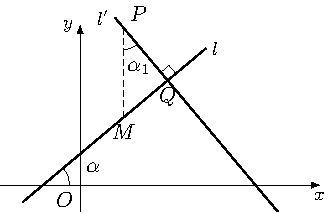
\includegraphics{1-34a.pdf}
  \subcaption{}\label{fig:1-34a}
  \end{minipage}
  \begin{minipage}[b]{0.48\linewidth}\centering
  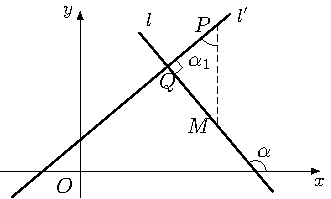
\includegraphics{1-34b.pdf}
  \subcaption{}\label{fig:1-34b}
  \end{minipage}
  \caption{}\label{fig:1-34}
\end{figure}

设点 $P$ 到直线 $l$ 的垂线为 $l'$ ,垂足为 $Q$。由 $l'\perp l$ 可知 $l'$ 的斜率为 $\dfrac{B}{A}(A \neq 0)$,根据点斜式可写出 $l'$ 的方程,并由 $l$ 与 $l'$ 的方程求出点 $Q$ 的坐标;由此即可根据两点距离公式求出 $|PQ|$,这就是点 $P$ 到直线 $l$ 的距离。

这个方法虽然思路自然,但是运算很繁,下面介绍另一种求法。

设 $A\neq 0$,$B\neq 0$,直线 $l$ 的倾斜角为 $\alpha$。过点 $P$ 作 $PM\parallel Oy$,那么 $PM$ 与 $l$ 相交于点 $M\,(x_1,y_1)$(\cref{fig:1-34})。
\begin{gather*}
\because \quad PM\parallel Oy,\\
\therefore \quad x_1=x_0.
\end{gather*}
代入直线 $l$ 的方程可得
\begin{gather*}
  y_1=-\frac{Ax_0+C}{B}.\\
  \begin{split}
  \therefore\quad |PM| & =|y_0-y_1|=\left|y_0+\frac{Ax_0+C}{B}\right|\\
                  & = \frac{|Ax_0+By_0+C|}{|B|}
  \end{split}
\end{gather*}

当 $\alpha<\ang{90}$ 时(如\cref{fig:1-34a}),$\alpha_1=\alpha$;

当 $\alpha>\ang{90}$ 时(如\cref{fig:1-34b}),$\alpha_1= \uppi-\alpha$,

所以,在两种情况下都有
\begin{gather*}
\tan^2\alpha_1=\tan^2\alpha=\frac{A^2}{B^2}.\\
\because \quad \alpha_1< \ang{90},\\
\begin{split}
  \cos\alpha_1&=\frac{1}{\sqrt{1+\tan^2\alpha_1}}=\frac{1}{\sqrt{1+\dfrac{A^2}{B^2}}}\\
   &=\frac{\left| B\right| }{\sqrt{{A}^{2} + {B}^{2}}}.\\
% \end{split}\\
% %
% % \[
% \begin{split}
  \therefore\quad |PQ|&=|PM|\cos\alpha_1\\
   &=\frac{|Ax_0+By_0+C|}{|B|} \cdot \frac{|B|}{\sqrt{A^2+B^2}}\\
   &=\frac{|Ax_0+By_0+C|}{\sqrt{A^2+B^2}}.
\end{split}
% \]
\end{gather*}

这样,我们就得到平面内一点 $P\,(x_0,y_0)$ 到一条直线 $Ax+By+C=0$ 的距离公式:
\[ \tcbhighmath{d = \frac{|Ax_0+By_0+C|}{\sqrt{A^2+B^2}}}. \]

如果 $A=0$ 或 $B=0$,上面的距离公式仍然成立。
但这时不需要利用公式就可以直接求出距离。

\begin{example}
  求点 $P_0\,(-1,2)$ 到直线 
  \begin{tasks}(2)
    \task $2x+y-10=0$;
    \task $3x=2$。
  \end{tasks}
  的距离。
\end{example}
\begin{solution}
  \begin{enumerate}[a)]
    \item 根据点到直线的距离公式,得
    \[ d=\frac{|2\times(-1)+1\times2-10|}{\sqrt{2^2+1^2}}=2\sqrt{5}\]
    \item 因为直线 $3x=2$ 平行于 $y$ 轴,所以
    \[d=\left|\frac{2}{3}-(-1)\right|=\frac{5}{3}\]
  \end{enumerate}
\end{solution}

\begin{example}
  求平行线 $2x-7y+8=0$ 和 $2x-7y-6=0$ 的距离。
\end{example}

\noindent
\begin{minipage}{0.55\linewidth}\parindent2em
\begin{solution}
  在直线 $2x-7y-6=0$ 上任取一点,例如取 $P\,(3,0)$(\cref{fig:1-35}),则两平行线的距离就是点 $P\,(3,0)$ 到直线 
  \[2x-7y+8=0\]
  的距离。
\end{solution}
\end{minipage}\hfill
\begin{minipage}{0.4\linewidth}\centering
\begin{figurehere}
  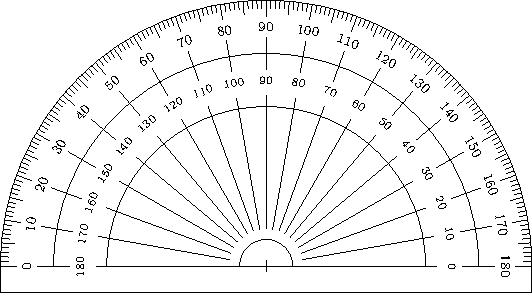
\includegraphics{1-35.pdf}
  \caption{}\label{fig:1-35}
\end{figurehere}
\end{minipage}

\medskip
因此,
\[
  d=\frac{|2\times3-7\times0+8|}{\sqrt{2^2+7^2}}=\frac{14}{\sqrt{53}}=\frac{14\sqrt{53}}{53}.
\]

\begin{Practice}
  \begin{question}
    \item 求坐标原点到下列直线的距离:
    \begin{tasks}(2)
      \task $3x+2y-26=0$;
      \task $x=y$。
    \end{tasks}
    \item 求下列点到直线的距离:
    \begin{tasks}(2)
      \task $A\,(-2,3)$,$3x+4y+3=0$;
      \task $B\,(1,0)$,$\sqrt{3}x+y-\sqrt{3}=0$;
      \task $C\,(1,-2)$,$4x+3y=0$。
    \end{tasks}
    \item 求下列两条平行线的距离:
    \begin{tasks}
      \task $2x+3y-8=0$,$2x+3y+18=0$;
      \task $3x+4y=10$,$3x+4y=0$。
    \end{tasks}
  \end{question}
\end{Practice}

\begin{Exercise}
  \begin{question}
    \item 已知直线分别满足下列条件,求直线的方程:
    \begin{tasks}
      \task 经过点 $A\,(3,2)$,且与直线 $4x+y-2=0$ 平行;
      \task 经过点 $B\,(3,0)$,且与直线 $2x+y-5=0$ 垂直;
      \task 经过点 $C\,(2,-3)$,且平行于过两点 $M\,(1,2)$ 和 $N\,(-1,-5)$ 的直线。
    \end{tasks}
    \item 设有两点 $A\,(7,-4)$、$B\,(-5,6)$,求线段 $AB$ 的垂直平分线的方程。
    \item 三角形三个顶点是 $A\,(4,0)$、$B\,(6,7)$、$C\,(0,3)$。求这个三角形的三条高所在直线的方程。
    \item 已知直线分别满足下列条件,求直线的方程:
    \begin{tasks}
      \task 斜率为 $-2$,且过两条直线 $3x-y+4=0$ 和 $x+y-4=0$ 的交点;
      \task 过两条直线 $x-2y+3=0$ 和 $x+2y-9=0$ 的交点和原点;
      \task 经过两条直线 $2x-3y+10=0$ 和 $3x+4y-2=0$ 的交点,且垂直于直线 $3x-2y+4=0$;
      \task 经过两条直线 $2x+y-8=0$ 和 $x-2y+1=0$ 的交点,且平行于直线 $4x-3y-7=0$;
      \task 经过直线 $y=2x+3$ 和 $3x-y+2=0$ 的交点,且垂直于第一条直线。
    \end{tasks}
    \item 直线 $ax+2y+8=0$,$4x+3y=10$ 和 $2x-y=10$ 相交于一点。求 $a$ 的值。
    \item 不解方程组,判定下列两个方程的直线的位置关系。
    \begin{tasks}(2)
      \task $\begin{cases} 2x+y=11,\\x+3y=18; \end{cases}$
      \task $\begin{cases} 2x-3y=4,\\4x-6y=8; \end{cases}$
      \task $\begin{cases} 3x+10y=16,\\6x+20y=7; \end{cases}$
      \task $\begin{cases} 4x+10y=12,\\6x-15y=18. \end{cases}$
    \end{tasks}
    \item 已知两条直线 $l_1:(3+m)x+4y=5-3m$,$l_2:2x+(5+m)y=8$。$m$ 为何值时,$l_1$ 与 $l_2$
    \begin{tasks}(3)
      \task 相交;
      \task 平行;
      \task 重合。
    \end{tasks}
    \item 讨论两条直线 $l_1:A_1x+B_1y+C_1=0$,$l_2:A_2x+B_2y+C_2=0$ 的位置关系:
    \begin{tasks}(2)
      \task 当 $B_1=0$、 $B_2\neq0$ 时,
      \task 当 $B_1=B_2=0$ 时。
    \end{tasks}
    \item 三角形的三个顶点是 $A\,(6,3)$、$B\,(9,3)$、$C\,(3,6)$。求它的三个内角的度数。
    \item 已知直线 $l$ 经过点 $P\,(2,1)$ ,且和直线 $5x+2y+3=0$ 的夹角等于 \ang{45}。求直线 $l$ 的方程。
    \item 光线从点 $M\,(-2,3)$ 射到 $x$ 轴上一点 $P\,(1,0)$ 后被 $x$ 轴反射。求反射光线所在直线的方程。
    \item 求点 $P\,(-5,7)$ 到直线 $12x+5y-3=0$ 的距离。
    \item 点 $A\,(a,6)$ 到直线 $3x-4y=2$ 的距离
    \begin{tasks}(2)
      \task 等于 4;
      \task 大于 4。
    \end{tasks}
    分别求 $a$ 的值。
    \item 求证:两条平行线 $Ax+By+C_1=0$ 与 $Ax+By+C_2=0$ 的距离是
    \[ d = \frac{|C_1-C_2|}{\sqrt{A^2+B^2}}. \]
    \item 求两条平行线 $3x-2y-1=0$ 和 $6x-4y+2=0$ 的距离。
  \end{question}
\end{Exercise}

\section*{小结}
\begin{enumerate}[C、,itemindent=4.5em]
  \item 在这一章里,我们首先研究了有向线段、两点的距离及线段的定比分点;接着又研究了直线方程的各种形式,并利用这些方程讨论了两条直线的位置关系和两条直线所成的角、点到直线的距离。这种通过方程研究图形性质的方法就是解析法。解析法揭示了数学中“数”和“形”的内在联系。
  \item 有向线段的数量、两点的距离与定比分点等公式是解析几何的基本公式。在用解析法研究点的轨迹问题时,经常用到这些公式。
  \item 本章介绍了点斜式、斜截式;两点式、截距式等直线方程的特殊形式,并研究了直线方程的一般式,这些直线的方程都是二元一次方程。每一个二元一次方程都表示一条直线;反之,表示每一条直线的方程都是二元一次方程。但是表示同一条直线的方程形式却不是唯一的,不过它们都可以通过方程的同解变形互化,可以看作是同一个方程。就这个意义来说,直线和二元一次方程是一一对应的。
  \item 直线的斜率和截距是表示直线位置的重要特征数值,通过它们可以判定两条直线的位置关系:平行、相交(包括垂直)及重合。
  
  在斜截式 $y=kx+b$ 中,如果 $k$ 固定,$b$ 取不同的值时,我们得到一组平行的直线;在点斜式方程 $y-y_0=k(x-x_0)$ 中,$k$ 取不同的值时,则得到过定点 $A\,(x_0,y_0)$ 的一组直线。
  \item 二元一次不等式表示区域和直线型经验公式在生产与科学研究中都常常用到。利用二元一次不等式表示的区域,我们还可以确定一个点与直线的位置关系。把点 $P\,(x_0,y_0)$ 的坐标代入直线方程 $Ax+By+C=0$ 的左边,由 $Ax+By+C$ 的值的正负可以确定点 $P$ 是在该直线的上方还是下方。
  \item 在研究了直线方程的各种形式之后,本章还研究了两条直线的交点、夹角以及点到直线的距离等问题。我们除了要掌握这些问题的结论外,还应注意学习通过代数方程研究几何性质的方法。
\end{enumerate}

\chapter*{复习参考题\chinese{chapter}}
\section*{A 组}
\begin{question}
  \item 已知 $\triangle ABC$ 顶点的坐标是 $A\,(2,3)$、$B\,(5,3)$、$C\,(2,7)$。求 $\angle A$ 的平分线长及所在直线的方程。
  \item 已知矩形的顶点为 $O\,(0,0)$、$A\,(8,0)$、$B\,(0,5)$。试用两种方法求两条对角线所在直线的方程。
  \item 用两种方法证明:三点 $A\,(-2,12)$、$B\,(1,3)$、$A\,(4,-6)$ 在同一条直线上。
  \item 求直线 $2x-5y-10=0$ 和坐标轴所围成的三角形的面积。
  \item 求经过点 $A\,(-3,4)$,并且在两轴上截距的和等于 12 的直线的方程。
  \item 在 $x$,$y$ 的坐标都不小于 0 的整数点中,求满足 $x+y\leqslant 4$ 的点的个数。
  \item 一定量的气体,在一定压强下体积 $V$(\unit{cm^3})和温度 $T$(\unit{\celsius})之间关系的实验数据如下:
  \begin{tablehere}
    \begin{tblr}{colspec={c*{6}{X[c]}},vline{2}=0.8pt}
      $T$(\unit{\celsius})& 20 & 30 & 40 & 50 & 60 & 70 \\
      $V$(\unit{cm^3})    & 106.5 & 110.9 & 114.0 & 117.2 & 121.2 & 124.7 \\
    \end{tblr}
  \end{tablehere}
  用选点法求出 $V$ 与 $T$ 间的经验公式。
  \item 一个 \qty{10}{\ohm} 的电阻,使用不同的电压通电,量得电流数值如下:
  \begin{tablehere}
    \begin{minipage}{\linewidth}
    \begin{tblr}{colspec={c*{6}{X[c]}},vline{2}=0.8pt}
      电压 $V$(\unit{V})& 5 & 10 & 15 & 20 & 25 & 30 \\
      电流 $I$(\unit{A})& 0.55 & 1.14 & 1.45 & 2.10 & 2.45 & 3.10 \\
    \end{tblr}
    \end{minipage}
  \end{tablehere}
  用平均值法求出 $I$ 与 $V$ 间的经验公式。
  \item 已知平行四边形两条边所在直线的方程是
  \[ x+y-1=0,\quad 3x-y+4=0,\]
  它的对角线的交点是 $M\,(3,3)$。求这个平行四边形其他两边的方程。
  \item 直线 $(3a+2)x+(1-4a)y+8=0$ 和 $(5a-2)x+(a+4)y-7=0$ 互相垂直。求 $a$ 的值。
  \item $ABCD$ 是正方形,$E$、$F$、$G$、$H$ 分别是边 $AB$、$BC$、$CD$、$DA$ 的中点。求证:
  \begin{tasks}
    \task 线段 $AF$、$BG$、$CH$、$DE$ 围成一个正方形;
    \task 这个正方形的面积是原正方形面积的 $\dfrac{1}{5}$。
  \end{tasks}
  \item 解答:
  \begin{enumerate}[a),itemindent=1.5em]
    \item 当 $a$ 为何值时,下列两方程的直线平行:
    \begin{tasks}[label=\roman*)]
      \task $ax-5y=9$,$2x-3y=15$;
      \task $x+2ay-1=0$,$(3a-1)x-ay-1=0$;
      \task $2x+3y=a$,$4x+6y-3=0$。
    \end{tasks}
    \item 当 $m$、$n$ 各为何值时,下列两方程的直线重合:
    \begin{tasks}[label=\roman*)]
      \task $x+2y=4$,$mx+y=n$;
      \task $mx+10y=2$,$3x+(n-1)y=-1$。
    \end{tasks}
    \item 当 $a$ 为何值时,下列两方程的直线互相垂直:
    \begin{tasks}[label=\roman*)]
      \task $4ax+y=1$,$(1-a)x+y=-1$;
      \task $2x+ay=2$,$ax+2y=1$。
    \end{tasks}
  \end{enumerate}
  \item 已知两条直线 $l_1:x+(1+m)y=2-m$,$l_2:2mx+4y=-16$。$m$ 为何值时,$l_1$ 与 $l_2$
  \begin{tasks}(3)
    \task 相交;
    \task 平行;
    \task 重合。
  \end{tasks}
  \item 求两条平行直线 $3x+4y-12=0$ 和 $6x+8y+11=0$ 的距离。
  \item 求平行于直线 $x-y-2=0$ 且与它的距离为 $2\sqrt{2}$ 的直线方程。
  \item 正方形的中心在 $C\,(-1,0)$,一条边所在的直线方程是 $x+3y-5=0$,求其他三边所在的直线方程。
\end{question}
\section*{B 组}
\begin{question}[resume]
  \item 已知: 直线 $l:Ax+By+C=0$($A\neq 0,\,B\neq 0$),点 $M\,(x_0,y_0)$。求证:
  \begin{tasks}
    \task 经过点 $M$ 且平行于直线 $l$ 的直线方程是 $A(x-x_0)+B(y-y_0)=0$;
    \task 经过点 $M$ 且垂直于直线 $l$ 的直线的方程是 \[\frac{x-x_0}{A}=\frac{y-y_0}{B}.\]
  \end{tasks}
  \item 已知平行直线 $3x+2y-6=0$ 与 $6x+4y-3=0$。求与它们等距离的平行线的方程。
  \item 一条光线从点 $M_0\,(5,3)$ 射出后,被直线 $l:x+y=1$ 反射,入射光线到直线 $l$ 的角为 $\beta$。已知 $\tan\beta = 2$ ,求入射光线与反射光线所在直线的方程。
  \item 直线 $l_1$、$l_2$、$l_3$ 的方程分别是
  \begin{align*}
    l_1 &: A_1x+B_1y+C_1 =0; \\
    l_2 &: A_2x+B_2y+C_2 =0; \\
    l_3 &: A_1x+B_1y+C_1 + \lambda(A_2x+B_2y+C_2) =0. 
  \end{align*}
  如果当 
  \begin{tasks}(2)
    \task $l_1$ 和 $l_2$ 相交;
    \task $l_1$ 和 $l_2$ 平行
  \end{tasks}
  时,直线 $l_3$ 和 $l_1$、$l_2$ 的位置关系如何?
  \item\label{exec:1t-21} 山顶上有高 $h$ 的塔 $BC$,从塔顶 $B$ 测得地面上一点 $A$ 的俯角是 $\alpha$,从塔底 $C$ 测得点 $A$ 的俯角是 $\beta$,用解析法求山高 $H$。
  \begin{figurehere}
    \begin{minipage}{\linewidth}\centering
      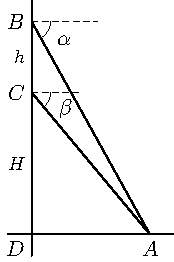
\includegraphics{1t-21.pdf}
    \caption*{(第~\ref{exec:1t-21}~题)}
    \end{minipage}
  \end{figurehere}
  \item 过两点 $A\,(-3,2)$ 和 $B\,(6,1)$ 的直线与直线 $x+3y-6=0$ 交于点 $P$。求点 $P$ 分 $\overline{AB}$ 所成的比。
\end{question}